% **************************************************************************************************************
% A Classic Thesis Style
% An Homage to The Elements of Typographic Style
%
% Copyright (C) 2015 André Miede http://www.miede.de
%
% If you like the style then I would appreciate a postcard. My address 
% can be found in the file ClassicThesis.pdf. A collection of the 
% postcards I received so far is available online at 
% http://postcards.miede.de
%
% License:
% This program is free software; you can redistribute it and/or modify
% it under the terms of the GNU General Public License as published by
% the Free Software Foundation; either version 2 of the License, or
% (at your option) any later version.
%
% This program is distributed in the hope that it will be useful,
% but WITHOUT ANY WARRANTY; without even the implied warranty of
% MERCHANTABILITY or FITNESS FOR A PARTICULAR PURPOSE.  See the
% GNU General Public License for more details.
%
% You should have received a copy of the GNU General Public License
% along with this program; see the file COPYING.  If not, write to
% the Free Software Foundation, Inc., 59 Temple Place - Suite 330,
% Boston, MA 02111-1307, USA.
%
% **************************************************************************************************************
\DeclareMathAlphabet{\mathcal}{OMS}{cmsy}{m}{n}
\RequirePackage{fix-cm} % fix some latex issues see: http://texdoc.net/texmf-dist/doc/latex/base/fixltx2e.pdf
\documentclass[ twoside,openright,titlepage,numbers=noenddot,headinclude,%1headlines,% letterpaper a4paper
                footinclude=true,cleardoublepage=empty,abstractoff, % <--- obsolete, remove (todo)
                BCOR=5mm,paper=a4,fontsize=11pt,%11pt,a4paper,%
                ngerman,american,%
                ]{scrreprt}

%********************************************************************
% Note: Make all your adjustments in here
%*******************************************************
% ****************************************************************************************************
% classicthesis-config.tex 
% formerly known as loadpackages.sty, classicthesis-ldpkg.sty, and classicthesis-preamble.sty 
% Use it at the beginning of your ClassicThesis.tex, or as a LaTeX Preamble 
% in your ClassicThesis.{tex,lyx} with % ****************************************************************************************************
% classicthesis-config.tex 
% formerly known as loadpackages.sty, classicthesis-ldpkg.sty, and classicthesis-preamble.sty 
% Use it at the beginning of your ClassicThesis.tex, or as a LaTeX Preamble 
% in your ClassicThesis.{tex,lyx} with % ****************************************************************************************************
% classicthesis-config.tex 
% formerly known as loadpackages.sty, classicthesis-ldpkg.sty, and classicthesis-preamble.sty 
% Use it at the beginning of your ClassicThesis.tex, or as a LaTeX Preamble 
% in your ClassicThesis.{tex,lyx} with \input{classicthesis-config}
% ****************************************************************************************************  
% If you like the classicthesis, then I would appreciate a postcard. 
% My address can be found in the file ClassicThesis.pdf. A collection 
% of the postcards I received so far is available online at 
% http://postcards.miede.de
% ****************************************************************************************************


% ****************************************************************************************************
% 0. Set the encoding of your files. UTF-8 is the only sensible encoding nowadays. If you can't read
% äöüßáéçèê∂åëæƒÏ€ then change the encoding setting in your editor, not the line below. If your editor
% does not support utf8 use another editor!
% ****************************************************************************************************
\PassOptionsToPackage{utf8}{inputenc}
	\usepackage{inputenc}

% ****************************************************************************************************
% 1. Configure classicthesis for your needs here, e.g., remove "drafting" below 
% in order to deactivate the time-stamp on the pages
% ****************************************************************************************************
\PassOptionsToPackage{eulerchapternumbers,listings,drafting,%
					 pdfspacing,%floatperchapter,%linedheaders,%
					 subfig,beramono,eulermath,parts}{classicthesis}                                        
% ********************************************************************
% Available options for classicthesis.sty 
% (see ClassicThesis.pdf for more information):
% drafting
% parts nochapters linedheaders
% eulerchapternumbers beramono eulermath pdfspacing minionprospacing
% tocaligned dottedtoc manychapters
% listings floatperchapter subfig
% ********************************************************************


% ****************************************************************************************************
% 2. Personal data and user ad-hoc commands
% ****************************************************************************************************
\newcommand{\myTitle}{Creating a Bytecode Virtual Machine in C\xspace}
\newcommand{\mySubtitle}{A Level Computer Science\xspace}
\newcommand{\myDegree}{Non Assessed Examination (NEA)\xspace}
\newcommand{\myName}{Zaahir Ali\xspace}
\newcommand{\myProf}{Mr. D Travi\xspace}
\newcommand{\myOtherProf}{Put name here\xspace}
\newcommand{\mySupervisor}{Put name here\xspace}
\newcommand{\myFaculty}{Put data here\xspace}
\newcommand{\myDepartment}{Put data here\xspace}
\newcommand{\myUni}{The Royal Grammar School\xspace}
\newcommand{\myLocation}{High Wycombe\xspace}
\newcommand{\myTime}{September 2023\xspace}
\newcommand{\myVersion}{version 4.2\xspace}

% ********************************************************************
% Setup, finetuning, and useful commands
% ********************************************************************
\newcounter{dummy} % necessary for correct hyperlinks (to index, bib, etc.)
\newlength{\abcd} % for ab..z string length calculation
\providecommand{\mLyX}{L\kern-.1667em\lower.25em\hbox{Y}\kern-.125emX\@}
\newcommand{\ie}{i.\,e.}
\newcommand{\Ie}{I.\,e.}
\newcommand{\eg}{e.\,g.}
\newcommand{\Eg}{E.\,g.} 
% ****************************************************************************************************


% ****************************************************************************************************
% 3. Loading some handy packages
% ****************************************************************************************************
% ******************************************************************** 
% Packages with options that might require adjustments
% ******************************************************************** 
%\PassOptionsToPackage{ngerman,american}{babel}   % change this to your language(s)
% Spanish languages need extra options in order to work with this template
%\PassOptionsToPackage{spanish,es-lcroman}{babel}
	\usepackage{babel}                  

\usepackage{csquotes}
\PassOptionsToPackage{%
    %backend=biber, %instead of bibtex
	backend=bibtex8,bibencoding=ascii,%
	language=auto,%
	style=numeric-comp,%
    %style=authoryear-comp, % Author 1999, 2010
    %bibstyle=authoryear,dashed=false, % dashed: substitute rep. author with ---
    sorting=nyt, % name, year, title
    maxbibnames=10, % default: 3, et al.
    %backref=true,%
    natbib=true % natbib compatibility mode (\citep and \citet still work)
}{biblatex}
    \usepackage{biblatex}

\PassOptionsToPackage{fleqn}{amsmath}       % math environments and more by the AMS 
    \usepackage{amsmath}

% ******************************************************************** 
% General useful packages
% ******************************************************************** 
\PassOptionsToPackage{T1}{fontenc} % T2A for cyrillics
    \usepackage{fontenc}     
\usepackage{textcomp} % fix warning with missing font shapes
\usepackage{scrhack} % fix warnings when using KOMA with listings package          
\usepackage{xspace} % to get the spacing after macros right  
\usepackage{mparhack} % get marginpar right
\usepackage{fixltx2e} % fixes some LaTeX stuff --> since 2015 in the LaTeX kernel (see below)
%\usepackage[latest]{latexrelease} % will be used once available in more distributions (ISSUE #107)
\PassOptionsToPackage{printonlyused,smaller}{acronym} 
    \usepackage{acronym} % nice macros for handling all acronyms in the thesis
    %\renewcommand{\bflabel}[1]{{#1}\hfill} % fix the list of acronyms --> no longer working
    %\renewcommand*{\acsfont}[1]{\textsc{#1}} 
    \renewcommand*{\aclabelfont}[1]{\acsfont{#1}}
% ****************************************************************************************************


% ****************************************************************************************************
% 4. Setup floats: tables, (sub)figures, and captions
% ****************************************************************************************************
\usepackage{tabularx} % better tables
    \setlength{\extrarowheight}{3pt} % increase table row height
\newcommand{\tableheadline}[1]{\multicolumn{1}{c}{\spacedlowsmallcaps{#1}}}
\newcommand{\myfloatalign}{\centering} % to be used with each float for alignment
\usepackage{caption}
% Thanks to cgnieder and Claus Lahiri
% http://tex.stackexchange.com/questions/69349/spacedlowsmallcaps-in-caption-label
% [REMOVED DUE TO OTHER PROBLEMS, SEE ISSUE #82]    
%\DeclareCaptionLabelFormat{smallcaps}{\bothIfFirst{#1}{~}\MakeTextLowercase{\textsc{#2}}}
%\captionsetup{font=small,labelformat=smallcaps} % format=hang,
\captionsetup{font=small} % format=hang,
\usepackage{subfig}  
% ****************************************************************************************************


% ****************************************************************************************************
% 5. Setup code listings
% ****************************************************************************************************
\usepackage{listings} 
%\lstset{emph={trueIndex,root},emphstyle=\color{BlueViolet}}%\underbar} % for special keywords
\lstset{language=[LaTeX]Tex,%C++,
    morekeywords={PassOptionsToPackage,selectlanguage},
    keywordstyle=\color{RoyalBlue},%\bfseries,
    basicstyle=\small\ttfamily,
    %identifierstyle=\color{NavyBlue},
    commentstyle=\color{Green}\ttfamily,
    stringstyle=\rmfamily,
    numbers=none,%left,%
    numberstyle=\scriptsize,%\tiny
    stepnumber=5,
    numbersep=8pt,
    showstringspaces=false,
    breaklines=true,
    %frameround=ftff,
    %frame=single,
    belowcaptionskip=.75\baselineskip
    %frame=L
} 
% ****************************************************************************************************             


% ****************************************************************************************************
% 6. PDFLaTeX, hyperreferences and citation backreferences
% ****************************************************************************************************
% ********************************************************************
% Using PDFLaTeX
% ********************************************************************
\PassOptionsToPackage{pdftex,hyperfootnotes=false,pdfpagelabels}{hyperref}
    \usepackage{hyperref}  % backref linktocpage pagebackref
\pdfcompresslevel=9
\pdfadjustspacing=1 
\PassOptionsToPackage{pdftex}{graphicx}
    \usepackage{graphicx} 
 

% ********************************************************************
% Hyperreferences
% ********************************************************************
\hypersetup{%
    %draft, % = no hyperlinking at all (useful in b/w printouts)
    colorlinks=true, linktocpage=true, pdfstartpage=3, pdfstartview=FitV,%
    % uncomment the following line if you want to have black links (e.g., for printing)
    %colorlinks=false, linktocpage=false, pdfstartpage=3, pdfstartview=FitV, pdfborder={0 0 0},%
    breaklinks=true, pdfpagemode=UseNone, pageanchor=true, pdfpagemode=UseOutlines,%
    plainpages=false, bookmarksnumbered, bookmarksopen=true, bookmarksopenlevel=1,%
    hypertexnames=true, pdfhighlight=/O,%nesting=true,%frenchlinks,%
    urlcolor=webbrown, linkcolor=RoyalBlue, citecolor=webgreen, %pagecolor=RoyalBlue,%
    %urlcolor=Black, linkcolor=Black, citecolor=Black, %pagecolor=Black,%
    pdftitle={\myTitle},%
    pdfauthor={\textcopyright\ \myName, \myUni, \myFaculty},%
    pdfsubject={},%
    pdfkeywords={},%
    pdfcreator={pdfLaTeX},%
    pdfproducer={LaTeX with hyperref and classicthesis}%
}   

% ********************************************************************
% Setup autoreferences
% ********************************************************************
% There are some issues regarding autorefnames
% http://www.ureader.de/msg/136221647.aspx
% http://www.tex.ac.uk/cgi-bin/texfaq2html?label=latexwords
% you have to redefine the makros for the 
% language you use, e.g., american, ngerman
% (as chosen when loading babel/AtBeginDocument)
% ********************************************************************
\makeatletter
\@ifpackageloaded{babel}%
    {%
       \addto\extrasamerican{%
			\renewcommand*{\figureautorefname}{Figure}%
			\renewcommand*{\tableautorefname}{Table}%
			\renewcommand*{\partautorefname}{Part}%
			\renewcommand*{\chapterautorefname}{Chapter}%
			\renewcommand*{\sectionautorefname}{Section}%
			\renewcommand*{\subsectionautorefname}{Section}%
			\renewcommand*{\subsubsectionautorefname}{Section}%     
                }%
       \addto\extrasngerman{% 
			\renewcommand*{\paragraphautorefname}{Absatz}%
			\renewcommand*{\subparagraphautorefname}{Unterabsatz}%
			\renewcommand*{\footnoteautorefname}{Fu\"snote}%
			\renewcommand*{\FancyVerbLineautorefname}{Zeile}%
			\renewcommand*{\theoremautorefname}{Theorem}%
			\renewcommand*{\appendixautorefname}{Anhang}%
			\renewcommand*{\equationautorefname}{Gleichung}%        
			\renewcommand*{\itemautorefname}{Punkt}%
                }%  
            % Fix to getting autorefs for subfigures right (thanks to Belinda Vogt for changing the definition)
            \providecommand{\subfigureautorefname}{\figureautorefname}%             
    }{\relax}
\makeatother


% ****************************************************************************************************
% 7. Last calls before the bar closes
% ****************************************************************************************************
% ********************************************************************
% Development Stuff
% ********************************************************************
\listfiles
%\PassOptionsToPackage{l2tabu,orthodox,abort}{nag}
%   \usepackage{nag}
%\PassOptionsToPackage{warning, all}{onlyamsmath}
%   \usepackage{onlyamsmath}

% ********************************************************************
% Last, but not least...
% ********************************************************************
\usepackage{classicthesis} 
% ****************************************************************************************************


% ****************************************************************************************************
% 8. Further adjustments (experimental)
% ****************************************************************************************************
% ********************************************************************
% Changing the text area
% ********************************************************************
%\linespread{1.05} % a bit more for Palatino
%\areaset[current]{312pt}{761pt} % 686 (factor 2.2) + 33 head + 42 head \the\footskip
%\setlength{\marginparwidth}{7em}%
%\setlength{\marginparsep}{2em}%

% ********************************************************************
% Using different fonts
% ********************************************************************
%\usepackage[oldstylenums]{kpfonts} % oldstyle notextcomp
%\usepackage[osf]{libertine}
%\usepackage[light,condensed,math]{iwona}
%\renewcommand{\sfdefault}{iwona}
%\usepackage{lmodern} % <-- no osf support :-(
%\usepackage{cfr-lm} % 
%\usepackage[urw-garamond]{mathdesign} <-- no osf support :-(
%\usepackage[default,osfigures]{opensans} % scale=0.95 
%\usepackage[sfdefault]{FiraSans}
% ****************************************************************************************************

% ****************************************************************************************************  
% If you like the classicthesis, then I would appreciate a postcard. 
% My address can be found in the file ClassicThesis.pdf. A collection 
% of the postcards I received so far is available online at 
% http://postcards.miede.de
% ****************************************************************************************************


% ****************************************************************************************************
% 0. Set the encoding of your files. UTF-8 is the only sensible encoding nowadays. If you can't read
% äöüßáéçèê∂åëæƒÏ€ then change the encoding setting in your editor, not the line below. If your editor
% does not support utf8 use another editor!
% ****************************************************************************************************
\PassOptionsToPackage{utf8}{inputenc}
	\usepackage{inputenc}

% ****************************************************************************************************
% 1. Configure classicthesis for your needs here, e.g., remove "drafting" below 
% in order to deactivate the time-stamp on the pages
% ****************************************************************************************************
\PassOptionsToPackage{eulerchapternumbers,listings,drafting,%
					 pdfspacing,%floatperchapter,%linedheaders,%
					 subfig,beramono,eulermath,parts}{classicthesis}                                        
% ********************************************************************
% Available options for classicthesis.sty 
% (see ClassicThesis.pdf for more information):
% drafting
% parts nochapters linedheaders
% eulerchapternumbers beramono eulermath pdfspacing minionprospacing
% tocaligned dottedtoc manychapters
% listings floatperchapter subfig
% ********************************************************************


% ****************************************************************************************************
% 2. Personal data and user ad-hoc commands
% ****************************************************************************************************
\newcommand{\myTitle}{Creating a Bytecode Virtual Machine in C\xspace}
\newcommand{\mySubtitle}{A Level Computer Science\xspace}
\newcommand{\myDegree}{Non Assessed Examination (NEA)\xspace}
\newcommand{\myName}{Zaahir Ali\xspace}
\newcommand{\myProf}{Mr. D Travi\xspace}
\newcommand{\myOtherProf}{Put name here\xspace}
\newcommand{\mySupervisor}{Put name here\xspace}
\newcommand{\myFaculty}{Put data here\xspace}
\newcommand{\myDepartment}{Put data here\xspace}
\newcommand{\myUni}{The Royal Grammar School\xspace}
\newcommand{\myLocation}{High Wycombe\xspace}
\newcommand{\myTime}{September 2023\xspace}
\newcommand{\myVersion}{version 4.2\xspace}

% ********************************************************************
% Setup, finetuning, and useful commands
% ********************************************************************
\newcounter{dummy} % necessary for correct hyperlinks (to index, bib, etc.)
\newlength{\abcd} % for ab..z string length calculation
\providecommand{\mLyX}{L\kern-.1667em\lower.25em\hbox{Y}\kern-.125emX\@}
\newcommand{\ie}{i.\,e.}
\newcommand{\Ie}{I.\,e.}
\newcommand{\eg}{e.\,g.}
\newcommand{\Eg}{E.\,g.} 
% ****************************************************************************************************


% ****************************************************************************************************
% 3. Loading some handy packages
% ****************************************************************************************************
% ******************************************************************** 
% Packages with options that might require adjustments
% ******************************************************************** 
%\PassOptionsToPackage{ngerman,american}{babel}   % change this to your language(s)
% Spanish languages need extra options in order to work with this template
%\PassOptionsToPackage{spanish,es-lcroman}{babel}
	\usepackage{babel}                  

\usepackage{csquotes}
\PassOptionsToPackage{%
    %backend=biber, %instead of bibtex
	backend=bibtex8,bibencoding=ascii,%
	language=auto,%
	style=numeric-comp,%
    %style=authoryear-comp, % Author 1999, 2010
    %bibstyle=authoryear,dashed=false, % dashed: substitute rep. author with ---
    sorting=nyt, % name, year, title
    maxbibnames=10, % default: 3, et al.
    %backref=true,%
    natbib=true % natbib compatibility mode (\citep and \citet still work)
}{biblatex}
    \usepackage{biblatex}

\PassOptionsToPackage{fleqn}{amsmath}       % math environments and more by the AMS 
    \usepackage{amsmath}

% ******************************************************************** 
% General useful packages
% ******************************************************************** 
\PassOptionsToPackage{T1}{fontenc} % T2A for cyrillics
    \usepackage{fontenc}     
\usepackage{textcomp} % fix warning with missing font shapes
\usepackage{scrhack} % fix warnings when using KOMA with listings package          
\usepackage{xspace} % to get the spacing after macros right  
\usepackage{mparhack} % get marginpar right
\usepackage{fixltx2e} % fixes some LaTeX stuff --> since 2015 in the LaTeX kernel (see below)
%\usepackage[latest]{latexrelease} % will be used once available in more distributions (ISSUE #107)
\PassOptionsToPackage{printonlyused,smaller}{acronym} 
    \usepackage{acronym} % nice macros for handling all acronyms in the thesis
    %\renewcommand{\bflabel}[1]{{#1}\hfill} % fix the list of acronyms --> no longer working
    %\renewcommand*{\acsfont}[1]{\textsc{#1}} 
    \renewcommand*{\aclabelfont}[1]{\acsfont{#1}}
% ****************************************************************************************************


% ****************************************************************************************************
% 4. Setup floats: tables, (sub)figures, and captions
% ****************************************************************************************************
\usepackage{tabularx} % better tables
    \setlength{\extrarowheight}{3pt} % increase table row height
\newcommand{\tableheadline}[1]{\multicolumn{1}{c}{\spacedlowsmallcaps{#1}}}
\newcommand{\myfloatalign}{\centering} % to be used with each float for alignment
\usepackage{caption}
% Thanks to cgnieder and Claus Lahiri
% http://tex.stackexchange.com/questions/69349/spacedlowsmallcaps-in-caption-label
% [REMOVED DUE TO OTHER PROBLEMS, SEE ISSUE #82]    
%\DeclareCaptionLabelFormat{smallcaps}{\bothIfFirst{#1}{~}\MakeTextLowercase{\textsc{#2}}}
%\captionsetup{font=small,labelformat=smallcaps} % format=hang,
\captionsetup{font=small} % format=hang,
\usepackage{subfig}  
% ****************************************************************************************************


% ****************************************************************************************************
% 5. Setup code listings
% ****************************************************************************************************
\usepackage{listings} 
%\lstset{emph={trueIndex,root},emphstyle=\color{BlueViolet}}%\underbar} % for special keywords
\lstset{language=[LaTeX]Tex,%C++,
    morekeywords={PassOptionsToPackage,selectlanguage},
    keywordstyle=\color{RoyalBlue},%\bfseries,
    basicstyle=\small\ttfamily,
    %identifierstyle=\color{NavyBlue},
    commentstyle=\color{Green}\ttfamily,
    stringstyle=\rmfamily,
    numbers=none,%left,%
    numberstyle=\scriptsize,%\tiny
    stepnumber=5,
    numbersep=8pt,
    showstringspaces=false,
    breaklines=true,
    %frameround=ftff,
    %frame=single,
    belowcaptionskip=.75\baselineskip
    %frame=L
} 
% ****************************************************************************************************             


% ****************************************************************************************************
% 6. PDFLaTeX, hyperreferences and citation backreferences
% ****************************************************************************************************
% ********************************************************************
% Using PDFLaTeX
% ********************************************************************
\PassOptionsToPackage{pdftex,hyperfootnotes=false,pdfpagelabels}{hyperref}
    \usepackage{hyperref}  % backref linktocpage pagebackref
\pdfcompresslevel=9
\pdfadjustspacing=1 
\PassOptionsToPackage{pdftex}{graphicx}
    \usepackage{graphicx} 
 

% ********************************************************************
% Hyperreferences
% ********************************************************************
\hypersetup{%
    %draft, % = no hyperlinking at all (useful in b/w printouts)
    colorlinks=true, linktocpage=true, pdfstartpage=3, pdfstartview=FitV,%
    % uncomment the following line if you want to have black links (e.g., for printing)
    %colorlinks=false, linktocpage=false, pdfstartpage=3, pdfstartview=FitV, pdfborder={0 0 0},%
    breaklinks=true, pdfpagemode=UseNone, pageanchor=true, pdfpagemode=UseOutlines,%
    plainpages=false, bookmarksnumbered, bookmarksopen=true, bookmarksopenlevel=1,%
    hypertexnames=true, pdfhighlight=/O,%nesting=true,%frenchlinks,%
    urlcolor=webbrown, linkcolor=RoyalBlue, citecolor=webgreen, %pagecolor=RoyalBlue,%
    %urlcolor=Black, linkcolor=Black, citecolor=Black, %pagecolor=Black,%
    pdftitle={\myTitle},%
    pdfauthor={\textcopyright\ \myName, \myUni, \myFaculty},%
    pdfsubject={},%
    pdfkeywords={},%
    pdfcreator={pdfLaTeX},%
    pdfproducer={LaTeX with hyperref and classicthesis}%
}   

% ********************************************************************
% Setup autoreferences
% ********************************************************************
% There are some issues regarding autorefnames
% http://www.ureader.de/msg/136221647.aspx
% http://www.tex.ac.uk/cgi-bin/texfaq2html?label=latexwords
% you have to redefine the makros for the 
% language you use, e.g., american, ngerman
% (as chosen when loading babel/AtBeginDocument)
% ********************************************************************
\makeatletter
\@ifpackageloaded{babel}%
    {%
       \addto\extrasamerican{%
			\renewcommand*{\figureautorefname}{Figure}%
			\renewcommand*{\tableautorefname}{Table}%
			\renewcommand*{\partautorefname}{Part}%
			\renewcommand*{\chapterautorefname}{Chapter}%
			\renewcommand*{\sectionautorefname}{Section}%
			\renewcommand*{\subsectionautorefname}{Section}%
			\renewcommand*{\subsubsectionautorefname}{Section}%     
                }%
       \addto\extrasngerman{% 
			\renewcommand*{\paragraphautorefname}{Absatz}%
			\renewcommand*{\subparagraphautorefname}{Unterabsatz}%
			\renewcommand*{\footnoteautorefname}{Fu\"snote}%
			\renewcommand*{\FancyVerbLineautorefname}{Zeile}%
			\renewcommand*{\theoremautorefname}{Theorem}%
			\renewcommand*{\appendixautorefname}{Anhang}%
			\renewcommand*{\equationautorefname}{Gleichung}%        
			\renewcommand*{\itemautorefname}{Punkt}%
                }%  
            % Fix to getting autorefs for subfigures right (thanks to Belinda Vogt for changing the definition)
            \providecommand{\subfigureautorefname}{\figureautorefname}%             
    }{\relax}
\makeatother


% ****************************************************************************************************
% 7. Last calls before the bar closes
% ****************************************************************************************************
% ********************************************************************
% Development Stuff
% ********************************************************************
\listfiles
%\PassOptionsToPackage{l2tabu,orthodox,abort}{nag}
%   \usepackage{nag}
%\PassOptionsToPackage{warning, all}{onlyamsmath}
%   \usepackage{onlyamsmath}

% ********************************************************************
% Last, but not least...
% ********************************************************************
\usepackage{classicthesis} 
% ****************************************************************************************************


% ****************************************************************************************************
% 8. Further adjustments (experimental)
% ****************************************************************************************************
% ********************************************************************
% Changing the text area
% ********************************************************************
%\linespread{1.05} % a bit more for Palatino
%\areaset[current]{312pt}{761pt} % 686 (factor 2.2) + 33 head + 42 head \the\footskip
%\setlength{\marginparwidth}{7em}%
%\setlength{\marginparsep}{2em}%

% ********************************************************************
% Using different fonts
% ********************************************************************
%\usepackage[oldstylenums]{kpfonts} % oldstyle notextcomp
%\usepackage[osf]{libertine}
%\usepackage[light,condensed,math]{iwona}
%\renewcommand{\sfdefault}{iwona}
%\usepackage{lmodern} % <-- no osf support :-(
%\usepackage{cfr-lm} % 
%\usepackage[urw-garamond]{mathdesign} <-- no osf support :-(
%\usepackage[default,osfigures]{opensans} % scale=0.95 
%\usepackage[sfdefault]{FiraSans}
% ****************************************************************************************************

% ****************************************************************************************************  
% If you like the classicthesis, then I would appreciate a postcard. 
% My address can be found in the file ClassicThesis.pdf. A collection 
% of the postcards I received so far is available online at 
% http://postcards.miede.de
% ****************************************************************************************************


% ****************************************************************************************************
% 0. Set the encoding of your files. UTF-8 is the only sensible encoding nowadays. If you can't read
% äöüßáéçèê∂åëæƒÏ€ then change the encoding setting in your editor, not the line below. If your editor
% does not support utf8 use another editor!
% ****************************************************************************************************
\PassOptionsToPackage{utf8}{inputenc}
	\usepackage{inputenc}

% ****************************************************************************************************
% 1. Configure classicthesis for your needs here, e.g., remove "drafting" below 
% in order to deactivate the time-stamp on the pages
% ****************************************************************************************************
\PassOptionsToPackage{eulerchapternumbers,listings,drafting,%
					 pdfspacing,%floatperchapter,%linedheaders,%
					 subfig,beramono,eulermath,parts}{classicthesis}                                        
% ********************************************************************
% Available options for classicthesis.sty 
% (see ClassicThesis.pdf for more information):
% drafting
% parts nochapters linedheaders
% eulerchapternumbers beramono eulermath pdfspacing minionprospacing
% tocaligned dottedtoc manychapters
% listings floatperchapter subfig
% ********************************************************************


% ****************************************************************************************************
% 2. Personal data and user ad-hoc commands
% ****************************************************************************************************
\newcommand{\myTitle}{Creating a Bytecode Virtual Machine in C\xspace}
\newcommand{\mySubtitle}{A Level Computer Science\xspace}
\newcommand{\myDegree}{Non Assessed Examination (NEA)\xspace}
\newcommand{\myName}{Zaahir Ali\xspace}
\newcommand{\myProf}{Mr. D Travi\xspace}
\newcommand{\myOtherProf}{Put name here\xspace}
\newcommand{\mySupervisor}{Put name here\xspace}
\newcommand{\myFaculty}{Put data here\xspace}
\newcommand{\myDepartment}{Put data here\xspace}
\newcommand{\myUni}{The Royal Grammar School\xspace}
\newcommand{\myLocation}{High Wycombe\xspace}
\newcommand{\myTime}{September 2023\xspace}
\newcommand{\myVersion}{version 4.2\xspace}

% ********************************************************************
% Setup, finetuning, and useful commands
% ********************************************************************
\newcounter{dummy} % necessary for correct hyperlinks (to index, bib, etc.)
\newlength{\abcd} % for ab..z string length calculation
\providecommand{\mLyX}{L\kern-.1667em\lower.25em\hbox{Y}\kern-.125emX\@}
\newcommand{\ie}{i.\,e.}
\newcommand{\Ie}{I.\,e.}
\newcommand{\eg}{e.\,g.}
\newcommand{\Eg}{E.\,g.} 
% ****************************************************************************************************


% ****************************************************************************************************
% 3. Loading some handy packages
% ****************************************************************************************************
% ******************************************************************** 
% Packages with options that might require adjustments
% ******************************************************************** 
%\PassOptionsToPackage{ngerman,american}{babel}   % change this to your language(s)
% Spanish languages need extra options in order to work with this template
%\PassOptionsToPackage{spanish,es-lcroman}{babel}
	\usepackage{babel}                  

\usepackage{csquotes}
\PassOptionsToPackage{%
    %backend=biber, %instead of bibtex
	backend=bibtex8,bibencoding=ascii,%
	language=auto,%
	style=numeric-comp,%
    %style=authoryear-comp, % Author 1999, 2010
    %bibstyle=authoryear,dashed=false, % dashed: substitute rep. author with ---
    sorting=nyt, % name, year, title
    maxbibnames=10, % default: 3, et al.
    %backref=true,%
    natbib=true % natbib compatibility mode (\citep and \citet still work)
}{biblatex}
    \usepackage{biblatex}

\PassOptionsToPackage{fleqn}{amsmath}       % math environments and more by the AMS 
    \usepackage{amsmath}

% ******************************************************************** 
% General useful packages
% ******************************************************************** 
\PassOptionsToPackage{T1}{fontenc} % T2A for cyrillics
    \usepackage{fontenc}     
\usepackage{textcomp} % fix warning with missing font shapes
\usepackage{scrhack} % fix warnings when using KOMA with listings package          
\usepackage{xspace} % to get the spacing after macros right  
\usepackage{mparhack} % get marginpar right
\usepackage{fixltx2e} % fixes some LaTeX stuff --> since 2015 in the LaTeX kernel (see below)
%\usepackage[latest]{latexrelease} % will be used once available in more distributions (ISSUE #107)
\PassOptionsToPackage{printonlyused,smaller}{acronym} 
    \usepackage{acronym} % nice macros for handling all acronyms in the thesis
    %\renewcommand{\bflabel}[1]{{#1}\hfill} % fix the list of acronyms --> no longer working
    %\renewcommand*{\acsfont}[1]{\textsc{#1}} 
    \renewcommand*{\aclabelfont}[1]{\acsfont{#1}}
% ****************************************************************************************************


% ****************************************************************************************************
% 4. Setup floats: tables, (sub)figures, and captions
% ****************************************************************************************************
\usepackage{tabularx} % better tables
    \setlength{\extrarowheight}{3pt} % increase table row height
\newcommand{\tableheadline}[1]{\multicolumn{1}{c}{\spacedlowsmallcaps{#1}}}
\newcommand{\myfloatalign}{\centering} % to be used with each float for alignment
\usepackage{caption}
% Thanks to cgnieder and Claus Lahiri
% http://tex.stackexchange.com/questions/69349/spacedlowsmallcaps-in-caption-label
% [REMOVED DUE TO OTHER PROBLEMS, SEE ISSUE #82]    
%\DeclareCaptionLabelFormat{smallcaps}{\bothIfFirst{#1}{~}\MakeTextLowercase{\textsc{#2}}}
%\captionsetup{font=small,labelformat=smallcaps} % format=hang,
\captionsetup{font=small} % format=hang,
\usepackage{subfig}  
% ****************************************************************************************************


% ****************************************************************************************************
% 5. Setup code listings
% ****************************************************************************************************
\usepackage{listings} 
%\lstset{emph={trueIndex,root},emphstyle=\color{BlueViolet}}%\underbar} % for special keywords
\lstset{language=[LaTeX]Tex,%C++,
    morekeywords={PassOptionsToPackage,selectlanguage},
    keywordstyle=\color{RoyalBlue},%\bfseries,
    basicstyle=\small\ttfamily,
    %identifierstyle=\color{NavyBlue},
    commentstyle=\color{Green}\ttfamily,
    stringstyle=\rmfamily,
    numbers=none,%left,%
    numberstyle=\scriptsize,%\tiny
    stepnumber=5,
    numbersep=8pt,
    showstringspaces=false,
    breaklines=true,
    %frameround=ftff,
    %frame=single,
    belowcaptionskip=.75\baselineskip
    %frame=L
} 
% ****************************************************************************************************             


% ****************************************************************************************************
% 6. PDFLaTeX, hyperreferences and citation backreferences
% ****************************************************************************************************
% ********************************************************************
% Using PDFLaTeX
% ********************************************************************
\PassOptionsToPackage{pdftex,hyperfootnotes=false,pdfpagelabels}{hyperref}
    \usepackage{hyperref}  % backref linktocpage pagebackref
\pdfcompresslevel=9
\pdfadjustspacing=1 
\PassOptionsToPackage{pdftex}{graphicx}
    \usepackage{graphicx} 
 

% ********************************************************************
% Hyperreferences
% ********************************************************************
\hypersetup{%
    %draft, % = no hyperlinking at all (useful in b/w printouts)
    colorlinks=true, linktocpage=true, pdfstartpage=3, pdfstartview=FitV,%
    % uncomment the following line if you want to have black links (e.g., for printing)
    %colorlinks=false, linktocpage=false, pdfstartpage=3, pdfstartview=FitV, pdfborder={0 0 0},%
    breaklinks=true, pdfpagemode=UseNone, pageanchor=true, pdfpagemode=UseOutlines,%
    plainpages=false, bookmarksnumbered, bookmarksopen=true, bookmarksopenlevel=1,%
    hypertexnames=true, pdfhighlight=/O,%nesting=true,%frenchlinks,%
    urlcolor=webbrown, linkcolor=RoyalBlue, citecolor=webgreen, %pagecolor=RoyalBlue,%
    %urlcolor=Black, linkcolor=Black, citecolor=Black, %pagecolor=Black,%
    pdftitle={\myTitle},%
    pdfauthor={\textcopyright\ \myName, \myUni, \myFaculty},%
    pdfsubject={},%
    pdfkeywords={},%
    pdfcreator={pdfLaTeX},%
    pdfproducer={LaTeX with hyperref and classicthesis}%
}   

% ********************************************************************
% Setup autoreferences
% ********************************************************************
% There are some issues regarding autorefnames
% http://www.ureader.de/msg/136221647.aspx
% http://www.tex.ac.uk/cgi-bin/texfaq2html?label=latexwords
% you have to redefine the makros for the 
% language you use, e.g., american, ngerman
% (as chosen when loading babel/AtBeginDocument)
% ********************************************************************
\makeatletter
\@ifpackageloaded{babel}%
    {%
       \addto\extrasamerican{%
			\renewcommand*{\figureautorefname}{Figure}%
			\renewcommand*{\tableautorefname}{Table}%
			\renewcommand*{\partautorefname}{Part}%
			\renewcommand*{\chapterautorefname}{Chapter}%
			\renewcommand*{\sectionautorefname}{Section}%
			\renewcommand*{\subsectionautorefname}{Section}%
			\renewcommand*{\subsubsectionautorefname}{Section}%     
                }%
       \addto\extrasngerman{% 
			\renewcommand*{\paragraphautorefname}{Absatz}%
			\renewcommand*{\subparagraphautorefname}{Unterabsatz}%
			\renewcommand*{\footnoteautorefname}{Fu\"snote}%
			\renewcommand*{\FancyVerbLineautorefname}{Zeile}%
			\renewcommand*{\theoremautorefname}{Theorem}%
			\renewcommand*{\appendixautorefname}{Anhang}%
			\renewcommand*{\equationautorefname}{Gleichung}%        
			\renewcommand*{\itemautorefname}{Punkt}%
                }%  
            % Fix to getting autorefs for subfigures right (thanks to Belinda Vogt for changing the definition)
            \providecommand{\subfigureautorefname}{\figureautorefname}%             
    }{\relax}
\makeatother


% ****************************************************************************************************
% 7. Last calls before the bar closes
% ****************************************************************************************************
% ********************************************************************
% Development Stuff
% ********************************************************************
\listfiles
%\PassOptionsToPackage{l2tabu,orthodox,abort}{nag}
%   \usepackage{nag}
%\PassOptionsToPackage{warning, all}{onlyamsmath}
%   \usepackage{onlyamsmath}

% ********************************************************************
% Last, but not least...
% ********************************************************************
\usepackage{classicthesis} 
% ****************************************************************************************************


% ****************************************************************************************************
% 8. Further adjustments (experimental)
% ****************************************************************************************************
% ********************************************************************
% Changing the text area
% ********************************************************************
%\linespread{1.05} % a bit more for Palatino
%\areaset[current]{312pt}{761pt} % 686 (factor 2.2) + 33 head + 42 head \the\footskip
%\setlength{\marginparwidth}{7em}%
%\setlength{\marginparsep}{2em}%

% ********************************************************************
% Using different fonts
% ********************************************************************
%\usepackage[oldstylenums]{kpfonts} % oldstyle notextcomp
%\usepackage[osf]{libertine}
%\usepackage[light,condensed,math]{iwona}
%\renewcommand{\sfdefault}{iwona}
%\usepackage{lmodern} % <-- no osf support :-(
%\usepackage{cfr-lm} % 
%\usepackage[urw-garamond]{mathdesign} <-- no osf support :-(
%\usepackage[default,osfigures]{opensans} % scale=0.95 
%\usepackage[sfdefault]{FiraSans}
% ****************************************************************************************************


%********************************************************************
% Bibliographies
%*******************************************************
\addbibresource{Bibliography.bib}
\addbibresource[label=ownpubs]{AMiede_Publications.bib}

%********************************************************************
% Hyphenation
%*******************************************************
%\hyphenation{put special hyphenation here}

% ********************************************************************
% GO!GO!GO! MOVE IT!
%*******************************************************
\usepackage[top=90pt,bottom=90pt,textwidth=400pt]{geometry}
\DeclareMathAlphabet{\mathcal}{OMS}{cmsy}{m}{n}
\begin{document}
\frenchspacing
\raggedbottom
\selectlanguage{american} % american ngerman
%\renewcommand*{\bibname}{new name}
%\setbibpreamble{}
\pagenumbering{roman}
\pagestyle{plain}
%*********************************************************\setmainfont{BaskervilleF}***********
% Frontmatter
%**********************************\setmainfont{BaskervilleF}*********************
%*******************************************************
% Little Dirty Titlepage
%*******************************************************
\thispagestyle{empty}
%\pdfbookmark[1]{Titel}{title}
%*******************************************************
\begin{center}
    \spacedlowsmallcaps{\myName} \\ \medskip                        

    \begingroup
        \color{Maroon}\spacedallcaps{\myTitle}
    \endgroup
\end{center}        

%*******************************************************
% Titlepage
%*******************************************************
\begin{titlepage}
    % if you want the titlepage to be centered, uncomment and fine-tune the line below (KOMA classes environment)
    \begin{addmargin}[-1cm]{-3cm}
    \begin{center}
        \large  

        \hfill

        \vfill

        \begingroup
            \color{Maroon}\spacedallcaps{\myTitle} \\ \bigskip
        \endgroup

        \spacedlowsmallcaps{\myName}

        \vfill

        
\includegraphics[width=6cm]{gfx/TFZsuperellipse_bw} \\ \medskip

        \mySubtitle \\ \medskip   
        %\myDegree \\
        %\myDepartment \\                            
        %\myFaculty \\
        %\myUni \\ \bigskip

        \myTime\ -- \myVersion

        \vfill                      

    \end{center}  
  \end{addmargin}       
\end{titlepage}   
\thispagestyle{empty}

\hfill

\vfill

\noindent\myName: \textit{\myTitle,} \mySubtitle, %\myDegree, 
\textcopyright\ \myTime

%\bigskip
%
%\noindent\spacedlowsmallcaps{Supervisors}: \\
%\myProf \\
%\myOtherProf \\ 
%\mySupervisor
%
%\medskip
%
%\noindent\spacedlowsmallcaps{Location}: \\
%\myLocation
%
%\medskip
%
%\noindent\spacedlowsmallcaps{Time Frame}: \\
%\myTime

\cleardoublepage%*******************************************************
% Dedication
%*******************************************************
\thispagestyle{empty}
%\phantomsection 
\refstepcounter{dummy}
\pdfbookmark[1]{Dedication}{Dedication}

\vspace*{3cm}

\begin{center}
    \emph{We ought not to be ashamed of appreciating the truth and of acquiring it wherever it comes from, even if it comes from peoples distant and nations different from us. For the seeker of truth nothing takes precedence over the truth, and there is no disparagement of the truth, nor belittling either of him who speaks it or of him who conveys it. The status of no one is diminished by the truth; rather does the truth ennoble all.} \\ \medskip
    --- Abū Yūsuf Ya‘qūb ibn Ishāq al-Kindī,\\ On First Philosophy (ca. 833-842 AD)    
\end{center}

% \medskip

% \begin{center}
%     Dedicated to the loving memory of Rudolf Miede. \\ \smallskip
%     1939\,--\,2005
% \end{center}
%\cleardoublepage\include{FrontBackmatter/Foreword}
\cleardoublepage%*******************************************************
% Abstract
%*******************************************************
%\renewcommand{\abstractname}{Abstract}
\pdfbookmark[1]{Abstract}{Abstract}
\begingroup
\let\clearpage\relax
\let\cleardoublepage\relax
\let\cleardoublepage\relax

\chapter*{Abstract}
This project is a bytecode virtual machine interpreter for the custom language C-, submitted as part of the requirements for the A Level Computer Science qualification. As part of the GUI requirements of the project we also include a playground for C-, where code is syntax highlighted, and can be executed while viewing the intermediate bytecode and \ac{VM} trace.
\endgroup			

\vfill
% \cleardoublepage%*******************************************************
% Publications
%*******************************************************
\pdfbookmark[1]{Publications}{publications}
\chapter*{Publications}\graffito{This is just an early --~and currently ugly~-- test!}
This might come in handy for PhD theses: some ideas and figures have appeared previously in the following publications:

%\noindent Put your publications from the thesis here. The packages \texttt{multibib} or \texttt{bibtopic} etc. can be used to handle multiple different bibliographies in your document.

\begin{refsection}[ownpubs]
    \small
    \nocite{*} % is local to to the enclosing refsection
    \printbibliography[heading=none]
\end{refsection}

\emph{Attention}: This requires a separate run of \texttt{bibtex} for your \texttt{refsection}, \eg, \texttt{ClassicThesis1-blx} for this file. You might also use \texttt{biber} as the backend for \texttt{biblatex}. See also \url{http://tex.stackexchange.com/questions/128196/problem-with-refsection}.
% \cleardoublepage%*******************************************************
% Acknowledgments
%*******************************************************
\pdfbookmark[1]{Acknowledgments}{acknowledgments}

\begin{flushright}{\slshape    
    We have seen that computer programming is an art, \\ 
    because it applies accumulated knowledge to the world, \\ 
    because it requires skill and ingenuity, and especially \\
    because it produces objects of beauty.} \\ \medskip
    --- \defcitealias{knuth:1974}{Donald E. Knuth}\citetalias{knuth:1974} \citep{knuth:1974}
\end{flushright}



\bigskip

\begingroup
\let\clearpage\relax
\let\cleardoublepage\relax
\let\cleardoublepage\relax
\chapter*{Acknowledgments}
Put your acknowledgments here.

Many thanks to everybody who already sent me a postcard!

Regarding the typography and other help, many thanks go to Marco 
Kuhlmann, Philipp Lehman, Lothar Schlesier, Jim Young, Lorenzo 
Pantieri and Enrico Gregorio\footnote{Members of GuIT (Gruppo 
Italiano Utilizzatori di \TeX\ e \LaTeX )}, J\"org Sommer, 
Joachim K\"ostler, Daniel Gottschlag, Denis Aydin, Paride 
Legovini, Steffen Prochnow, Nicolas Repp, Hinrich Harms, 
 Roland Winkler, Jörg Weber, Henri Menke, Claus Lahiri, 
 Clemens Niederberger, Stefano Bragaglia, Jörn Hees, 
 and the whole \LaTeX-community for support, ideas and 
 some great software.

\bigskip

\noindent\emph{Regarding \mLyX}: The \mLyX\ port was intially done by 
\emph{Nicholas Mariette} in March 2009 and continued by 
\emph{Ivo Pletikosi\'c} in 2011. Thank you very much for your 
work and for the contributions to the original style.


\endgroup




\pagestyle{scrheadings}
\cleardoublepage%*******************************************************
% Table of Contents
%*******************************************************
%\phantomsection
\refstepcounter{dummy}
\pdfbookmark[1]{\contentsname}{tableofcontents}
\setcounter{tocdepth}{2} % <-- 2 includes up to subsections in the ToC
\setcounter{secnumdepth}{3} % <-- 3 numbers up to subsubsections
\manualmark
\markboth{\spacedlowsmallcaps{\contentsname}}{\spacedlowsmallcaps{\contentsname}}
\tableofcontents 
\automark[section]{chapter}
\renewcommand{\chaptermark}[1]{\markboth{\spacedlowsmallcaps{#1}}{\spacedlowsmallcaps{#1}}}
\renewcommand{\sectionmark}[1]{\markright{\thesection\enspace\spacedlowsmallcaps{#1}}}
%*******************************************************
% List of Figures and of the Tables
%*******************************************************
\clearpage

\begingroup 
    \let\clearpage\relax
    \let\cleardoublepage\relax
    \let\cleardoublepage\relax
    %*******************************************************
    % List of Figures
    %*******************************************************    
    %\phantomsection 
    \refstepcounter{dummy}
    %\addcontentsline{toc}{chapter}{\listfigurename}
    \pdfbookmark[1]{\listfigurename}{lof}
    \listoffigures

    \vspace{8ex}

    %*******************************************************
    % List of Tables
    %*******************************************************
    %\phantomsection 
    \refstepcounter{dummy}
    %\addcontentsline{toc}{chapter}{\listtablename}
    \pdfbookmark[1]{\listtablename}{lot}
    \listoftables
        
    \vspace{8ex}
%   \newpage
    
    %*******************************************************
    % List of Listings
    %*******************************************************      
      %\phantomsection 
    \refstepcounter{dummy}
    %\addcontentsline{toc}{chapter}{\lstlistlistingname}
    \pdfbookmark[1]{\lstlistlistingname}{lol}
    \lstlistoflistings 

    \vspace{8ex}
       
    %*******************************************************
    % Acronyms
    %*******************************************************
    %\phantomsection 
    \refstepcounter{dummy}
    \pdfbookmark[1]{Acronyms}{acronyms}
    \markboth{\spacedlowsmallcaps{Acronyms}}{\spacedlowsmallcaps{Acronyms}}
    \chapter*{Acronyms}
    \begin{acronym}[UMLX]
        \acro{GC}{Garbage Collection}
        \acro{AST}{Abstract Syntax Tree}
        \acro{IR}{Intermediate Representation}
        \acro{VM}{Virtual Machine}
        \acro{JIT}{Just-In-Time}
        \acro{CPU}{Central Processing Unit}
        \acro{API}{Application Programming Interface}
        \acro{AOT}{Ahead Of Time}
    \end{acronym}                     
\endgroup

%********************************************************************
% Mainmatter
%*******************************************************
\cleardoublepage\pagenumbering{arabic}
%\setcounter{page}{90}
% use \cleardoublepage here to avoid problems with pdfbookmark
\cleardoublepage
\part{Design Overview}
% !TEX root = classicthesis.tex

%************************************************
\chapter{Introduction}\label{ch:introduction}
%************************************************

Engineers have been engaged in the development of programming languages since the inception of computing. Upon establishing communication with early computers, it became evident that this interaction posed significant challenges, prompting us to seek computational assistance. It is noteworthy that, despite the remarkable advancements in contemporary computing, characterized by computers that are a million times faster and equipped with substantially increased storage capacities, the foundational principles governing programming language construction have remained relatively consistent.

While the domain explored by language designers is expansive, the avenues they have pioneered within it are relatively circumscribed. While not all programming languages follow identical trajectories, with some opting for expedient shortcuts, they tend to share fundamental commonalities. This continuity is observed across the spectrum, from Rear Admiral Grace Hopper's seminal COBOL compiler to contemporary languages that transpile into JavaScript and are often accompanied by rudimentary documentation found in a solitary, modestly edited README nestled within a Git repository.

We can analogise the ascending of a mountain to serve to illustrate the process of language implementation. It commences at the base with the program in its raw source code form, consisting solely of alphanumeric characters. Each phase in the development process involves systematic analysis and transformation, culminating in a representation at a higher conceptual level that elucidates the intended semantics—the author's instructions for the computer. Upon reaching the summit, an all-encompassing perspective of the user's program is achieved, affording a comprehensive understanding of its intended function. Subsequently, the journey descends along the opposite side of the metaphorical mountain, progressively converting the highest-level representation into successively lower-level forms, drawing closer to a format amenable to execution by the \ac{CPU}.

Let us scale through these mountain trails and introduce certain points of interest. We start with the users source code.

\section{Dissecting a Programming Language}

\subsection{Parsing}

Parsing is done by a parser, a software device that takes input text and builds a data structure called the \ac{AST}, a hierachal structure that gives a systemic representation of the input text and checking it against the lexical grammar. This is either done through top-down parsing (also known as the primordial soup approach), a method where one first looks at the highest level of the parse tree and works down the parse tree by using the rewriting rules of a formal grammar, or through bottom-up parsing, a strategy that consists of a parser starting with the input and attempting to rewrite it to the start symbol. The parser attempts to locate the most basic elements of the input, and then the elements containing these and so on. 

This process starts with lexical analysis, also known as lexing, or more informally, scanning. In this step of the implementation process, a lexer (or scanner) takes in the linear stream of code and then breaks them down into small chunks, known as tokens. There are several different types of these tokens, ranging from special characters such as \verb+;+ (known as a seperator), to string literals \verb+("Hello, World!")+ and identifiers \verb+(max)+. For example, let us consider the following expression in the C programming language:

\begin{lstlisting}[language=C++]
z = x + y * 3;\end{lstlisting}

In this expression, the lexical analysis would produce the following tokens:

\begin{lstlisting}
[(identifier, z), (operator, =), (identifier, x), (operator, +), (identifier, y), (operator, *), (literal, 3), (separator, ;)]
\end{lstlisting}

These tokens are defined by the languages lexical grammar, consisting of regular expressions and define the possible lexemes of a token. If there's a mistake when comparing with the grammar rules of the language, the parser lets the programmer know by reporting a syntax error. Note that the parsing process is standard across compilers, interpreters and translators.   

\subsection{Static Analysis}

Now, the individual characteristics of each language start coming into play. At this point, we know the syntactic structure of the code, such as the nested expressions but not much else. 

In an expression like \verb{x + y{, we know we are adding \verb+x+ and \verb+y+, but we don’t know what those names refer to. Are they local variables or global? Where are they defined? This is where we use static analysis, where we can examine programs without executing them, compared to dynamic program analysis which we perform on programs during their execution. 

The analysis process starts with binding, also known as resolution. For every identifier within the code, we find out where they are defined and connect the two together, hence defining the scope of the identifier — the region of source code where a name actually refers to a declaration. 

In a statically typed language, a language where a variable is known at compile-time instead of at run-time, this is where type checking happens. If there's an error, for example \verb+x+ and \verb+y+ are of two different types which don't support addition, a type error is reported. Note that for dynamically typed languages, such as the one we will be building, the type checking is done during runtime. 


In our metaphorical mountain, this would be the peak, where we can see the entirity of the structure and meaning of the user's program. The semantic insight from this position can be stored in several places:

\begin{itemize}
	\item Most often, it's stored right back on the syntax tree itself as an attribute, extra fields in the tree nodes that aren't initialised during the parsing process but are inserted later during compilation.
	\item It may also be stored into a symbol table, a lookup table outside of the syntax tree that contains identifiers — the names of declarations and variables. 
	\item However the most powerful method is where we transform the tree into a new data structure that directly expresses the semantics of the code. This is known as an intermediate representation. 
\end{itemize}

This is the end of what's known as the front end of the implementation process. 

\subsection{Intermediate Representations}

We can think of each stage of the compilation process as aiming to organize the data representing the user's program in a fashion that makes the next stage of the process easier to implement. The front end of the compilation process is specific to the source language of the project, while the back end if concerned with the architecture of the machine that the program will run on. This is the ``middle end'' of the compilation process. 

At this point, code is stored in a \ac{IR} that isn't tied to either the source code or the destination architecture, and acts as a bridge, or interface, between the two languages. 

This means that if we want to support multiple source languages and target platforms we don't need to write multiple compilers for each possible combination of language and architecture, but instead, using a shared intermediate representation, we write one front end for each source langauge and one back end for each target architecture. This means we can mix and match, drastically reducing development time. However, this isn't the only reason we'd like to use a intermediate representation.

\subsection{Optimization}

Once we have a semantic overview of the user's program, we can substitute it with a different program that performs the same operations, just more efficiently, optimizing it. 

One form of this is constant folding; if one expression always evaluates to the same value (e.g it is constant) we can evaluate the expression at compile time and replace the code calculating the constant with the resulting number. If the original program was this:

\begin{lstlisting}[language=C++]
footballVolume = 4/3 * 3.14159 * (1)^3;
\end{lstlisting}

We could calculate this in the compiler and replace the code with:

\begin{lstlisting}[language=C++]
footballVolume = 4.18878667;
\end{lstlisting}

Another method is known as strength reducation, where expensive operations are replaced with equivalent but less expensive operations. Consider the following C code snippet: 

\begin{lstlisting}[language=C]
int i, sum = 0;
for (i = 1; i <= n; ++i) {
  sum += i;
}
printf("sum: %d\n", sum);

\end{lstlisting}

Assuming no arithmetic overflow, we can rewrite the code to be:

\begin{lstlisting}[language=C]
int sum = n * (1 + n) / 2;
printf("sum: %d\n", sum);
\end{lstlisting}

This makes use of the following mathematical standard summation for consecutive natural numbers: 
\begin{equation}\sum_{n=1}^i n = \frac{1}{2}n(n+1)\end{equation}
This same method of choosing more computationally efficient algorithms for performing operations is the key to strength reducation. However, note that the ``optimized'' version might actually be slower than the original version if \verb+n+ were sufficiently small and the particular hardware happens to be much faster at performing addition and looping operations than multiplication and division.

Furthermore, while the term ``optimization'' shares its root with ``optimal'', it is uncommon for the optimization process to yield a system that is genuinely optimal in all respects. Typically, a system can be optimized, not in an absolute sense, but rather in relation to a specific quality metric, which may conflict with other potential metrics. Consequently, the optimized system usually achieves optimality only within a particular application or for a specific target audience.

For instance, one might choose to reduce the execution time of a program, even if it results in increased memory consumption. In situations where conserving memory space is critical, deliberately opting for a slower algorithm may be a preferable trade-off. Frequently, there is no universally ideal design that can excel in all scenarios. Engineers must make calculated trade-offs to optimize the attributes that are most relevant to the task at hand. Several programming languages, such as CPython and Lua generate relatively unoptimized code and in exchange focus on performance effort during the runtime. 

\subsection{Code Generation}

After optimizing the user's source code, we move to coverting into machine code, a form that the machine can actually run. This is known as the generating code, where the code that is generated is usually some permutation of assembly code. 

Although somewhat unrelated, we should mention that when code generation takes place at runtime, such as in \ac{JIT} compilation, it is important that the process is efficient with respect to space and time. Despite its generally generating less efficient code, \ac{JIT} code generation can take advantage of profiling information that is available only at runtime.

This is the end of the middle end of the compilation process, and now part of the back end, the downward descent down our metaphorical mountain. We have gained an understanding of the user's program and now devolve the code, each step of the back end making the code more and more primitive so a simple \ac{CPU} can execute it. 

We can either produce instructions for a real \ac{CPU} or a virtual one. If we generate machine code for a real \ac{CPU} we are given an executeable that is loaded and executed directly on the chip by the machine's operating system. This results in fast code, but the generating process is significantly long due to complex pipelines, and a large and complicated instruction set. 
 
Furthermore, the produced executeable is also tied to the machine's architecture, say x86 or ARM, resulting in a lack of portability. To circumvent this, we can have our compiler produce virtual machine code, code that runs for some hypothetical machine. This is known as bytecode, since each instruction is often just a single byte long.

This synthetic set of instructions are designed to be based more around the properties of the source language rather than the the quirks of a computer architecture, sort of like a dense, binary encoding of the language’s low-level operations. 

\subsection{Virtual Machine}

However, this virtual code is useless without a chip that can understand it. We have two options, the first being a  `mini-compiler' for each real architecture we want out program to run to that converts the bytecode to native machine code for that language. This may seem counterproductive since we are trying to circumvent the architecture roadblock, but this step is relatively simple, and we able to retain the rest of the compiler across the machines we wish to support, meaning the bytecode essentially functions as a intermediate representation.

The other option would be a \ac{VM}, a program that emulates our hypothetical chip and supporting out virtual architecture at runtime. This implementation is slower than the prior method since every instruction must be simulated at runtime before executing, however in exchange a \ac{VM} offers simplicity and portability. 

There are two main types of virtual machines, system virtual machines (also known as full virtualisation \acsp{VM}) and process virtual machines. System virtual machines are a complete substitute for a real machine, provdiing the functionality to execute entire operating systems, while process virtual machines are designed to execute certain program in an isolated enviroment. This is the type we will be using throughout the project. 

\subsection{Runtime} 

We are finally at the end of the process of moulding the user's program into a form that we can run. The last step is running it. If we had compiled it to real machine code we would just tell the operating system to load and run the executeable file that is generated, however with bytecode we need to start the virtual machine and load the program through that. 

The runtime, often referred to as the runtime environment, is a crucial component in most programming languages, except for the most basic low-level ones. It provides essential services during program execution. One such service is memory management automation, which necessitates the presence of a garbage collector to reclaim unused memory.

Additionally, if the language supports ``instance of'' tests to determine object types, a mechanism for tracking the type of each object during runtime is required. The integration of these services into a program depends on the language's nature.

In the case of fully compiled languages, the code responsible for the runtime is directly inserted into the resulting executable. For example, in Go, each compiled application includes its own copy of Go's runtime, embedded within it. Conversely, languages that run within interpreters or virtual machines have the runtime environment residing in those environments. This operational model is commonly employed in languages like Java, Python, and JavaScript.

\section{Alternative Methods and Shortcuts}

This comprehensive journey covers every conceivable phase of implementation, and many languages do indeed traverse this entire route. However, there are a few  shortcuts and alternative paths available.

\subsection{Single-Pass Compilers}

A single-pass compiler, also known as a one-pass compiler is a compiler that passes through each compilation unit, such as a source file, only once and immediately transforms this into the final machine code that will be run. This means it skips the intermediate representation phase, does not allocate a syntax tree and does not reprocess the compilation unit in each sequential pass. In theory, this produces a smaller and faster processor, but compiler optimization is highly limited due to the limited scope of information available. Furthermore, many effective forms of compiler optimization, such as strength reduction, require multiple passes over structures such as a nested loop. 

\subsection{Tree-Walk Interpreters}

This approach functions by executing code right after it is parsed to an AST or using it to generate native code just-in-time. This is done by the interpreter traversing the syntax tree one branch at a time, evaluating each node as it parses. This again means each sentence only needs to be parsed once, and the \ac{AST} keeps the global program structure and relations (which is lost in bytecode representation). However, an \ac{AST} causes large overhead from visitng the tree (a less sequential representation causes traversal of more pointers) and because syntax nodes are useless during the process.

\subsection{Transpilers}

Creating a complete back end for a language is often a substantial undertaking. If we happen to possess a pre-existing, generic intermediate representation as our target, we can seamlessly integrate our front end with it. However, in cases where this isn't an option, we may find ourselves facing a daunting challenge.

Here's an alternative approach to consider: Instead of expending significant effort in the back end to transform the semantics into a lower-level target language, we can generate a string of valid source code for another language that shares a similar high-level nature with our own (compared to a traditional compiler which translates from high level to low level). This opens up the possibility of utilizing the existing compilation tools for that language to facilitate the transition from our elevated position to an executable form.

This methodology was once referred to as a ``source-to-source compiler'' or ``transcompiler.'' With the emergence of languages that compile to JavaScript for browser-based execution, it has gained a certain trendy reputation and is commonly known as a ``transpiler'' among the more hip programming circles.

\begin{figure}[h]
\centering
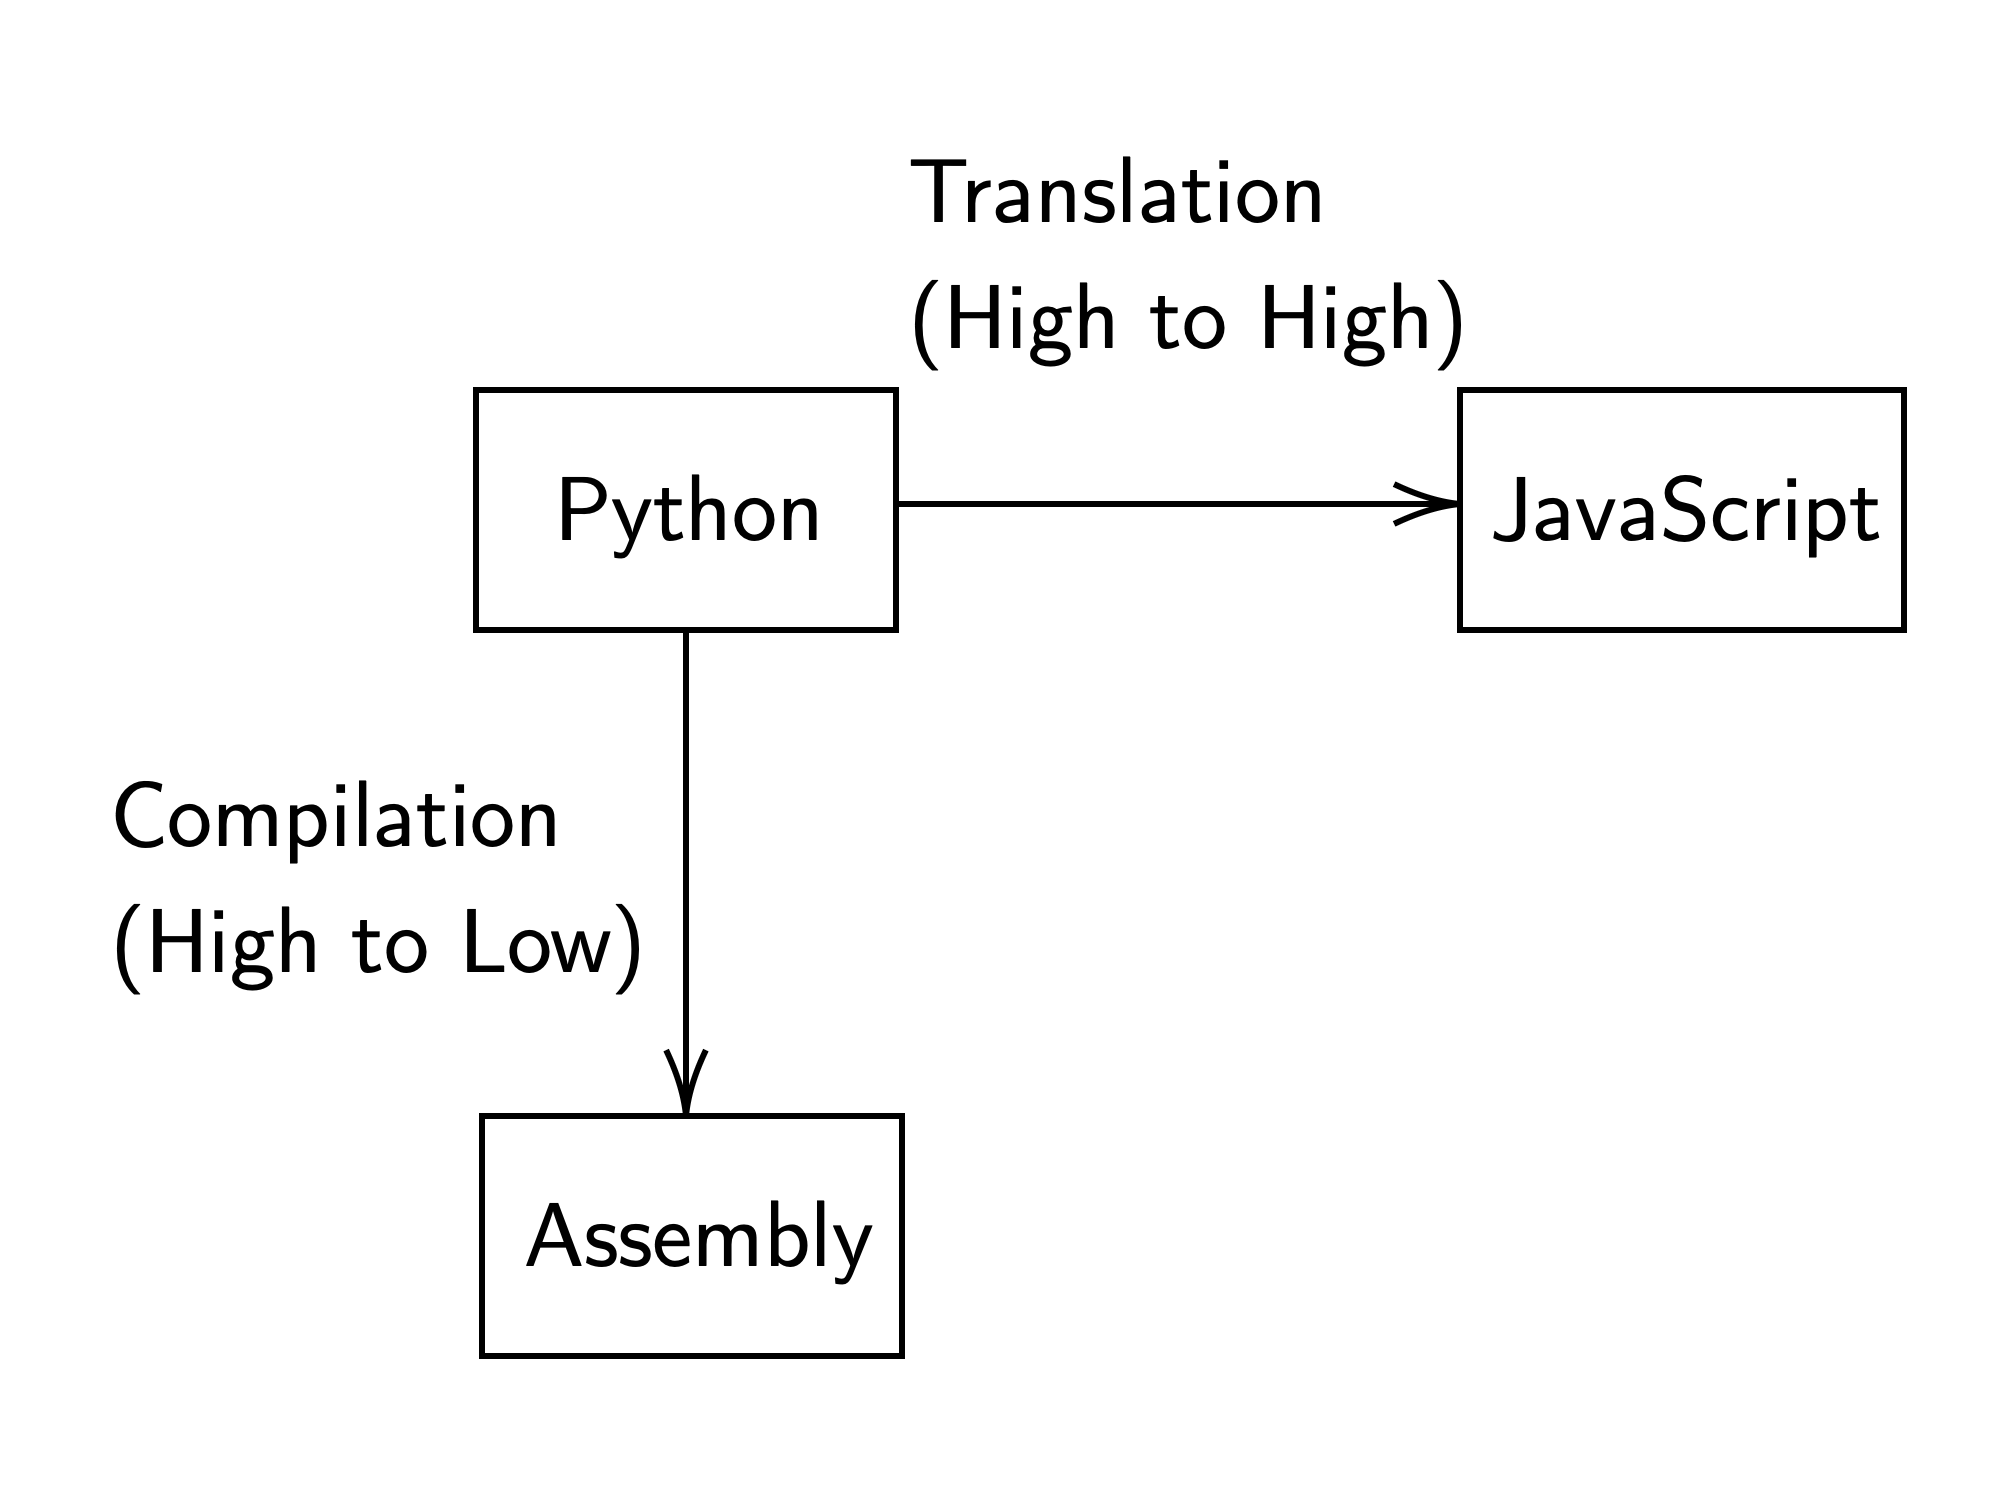
\includegraphics[width=0.75\textwidth]{gfx/transpiler.png}
\caption{Transpilers}
\end{figure}

Another valuable application of source-to-source compiling involves the translation of legacy code to adapt it to the next iteration of the underlying programming language or an \ac{API} that introduces changes, potentially breaking backward compatibility. This process also includes automatic code refactoring, which is useful when programs are impractically large or time-consuming to be done by hand. 

The parser of a transpiler is identical to other compilers, and analysis may be skipped if the source language is similar to the target language, meaning the corresponding syntax is output to the intended language straight after parsing. 

However, if the two language are not as syntactically similar, semantic analysis will be conducted, possibly with compiler optimizations as well, analogous to a full compiler. The difference comes at code generation, where instead of resulting in machine code, or some other binary language, we are produced with the program in the desired language which we can then run through that languages compilation process. 

\subsection{Just-In-Time Compilation}

This approach is more risky than those above, and involves compiling once the program is loaded at run-time on the user's machine, natively for the architecture of the end machine. This means you we can then compile for a machine architecture which was originally unknown and furtheremore at high speed. Although it is possible to compile the source code to machine code at run-time, often it is bytecode that is translated. 

This is actually a combination of two previous approaches in translation to machine code, \ac{AOT} compilation and interpretation, and \ac{JIT} tries to combine the advantges of both, albeit with some of the drawbacks. This compilation process results in speeds similar to pre-compiled code and flexibility comparitive to interpretation, hence it's use in dynamically typed languages. The overhead of this process however is a combination of the methods it draws upon, compiling and linking (not just interpreting)

At the highest levels \acsp{JIT} insert profiling hooks to understand which areas of the programs are most performance critical and over time recompile those with greater and more advanced optimizations. 

\section{Compilers and Interpreters}

We would like to start by defining a clear line between compilers and interpreters, which so far have almost been used interchangeably. In theory, a programming language can have both a compiler and interpreter, but in practice it often just implements just one. 

\subsection{Compilers}

To distinguish compilers from interpreters, it's crucial to understand that compilers are primarily concerned with translating source code into another form, typically a lower-level representation or machine code. This transformation allows for efficient execution of the program in the target environment. For example, when a high-level programming language like C++ is compiled, the source code is translated into machine code, and the result is an executable file. Importantly, the compilation process \textbf{does not} involve the direct execution of the program; instead, it produces an independent executable that can be run later. Consequently, once the compilation is complete, the original source code is no longer required to execute the program, making it suitable for distribution and deployment on various systems, as well as a greater security factor for preventing modification of the source code. This separation of compilation and execution is a key characteristic of compilers, as they focus on generating efficient stand-alone executables.

\subsection{Interpreters}

In contrast to compilers, interpreters operate by directly executing the source code ``on the fly''. When a programming language is implemented with an interpreter, it takes the source code as input and immediately begins executing it. This approach is often described as ``running from source'' because there is no intermediate step of generating a separate executable file. Instead, the interpreter interprets and executes each line or statement of the source code in real-time. This immediate execution can be advantageous for tasks like debugging, as errors are reported as they occur in the source code. However, it can also be less efficient than compiled code since the interpreter must repeatedly analyze and execute the code line by line. Interpreters are commonly used in scripting languages like Python and JavaScript, where rapid development and platform independence are more critical than raw execution speed.

An example of a language utilizing both implementations is CPython, which from the users perspective seems like as an interpreter — they can clearly see the program run from source. However, under the hood the code is parsed and converted into an internal bytecode format, which is then executed within the \ac{VM}, which is compiler like. We illustrate some other lagnuages and whether they use a compiler, interpreter or both:

\begin{figure}[h]
\centering
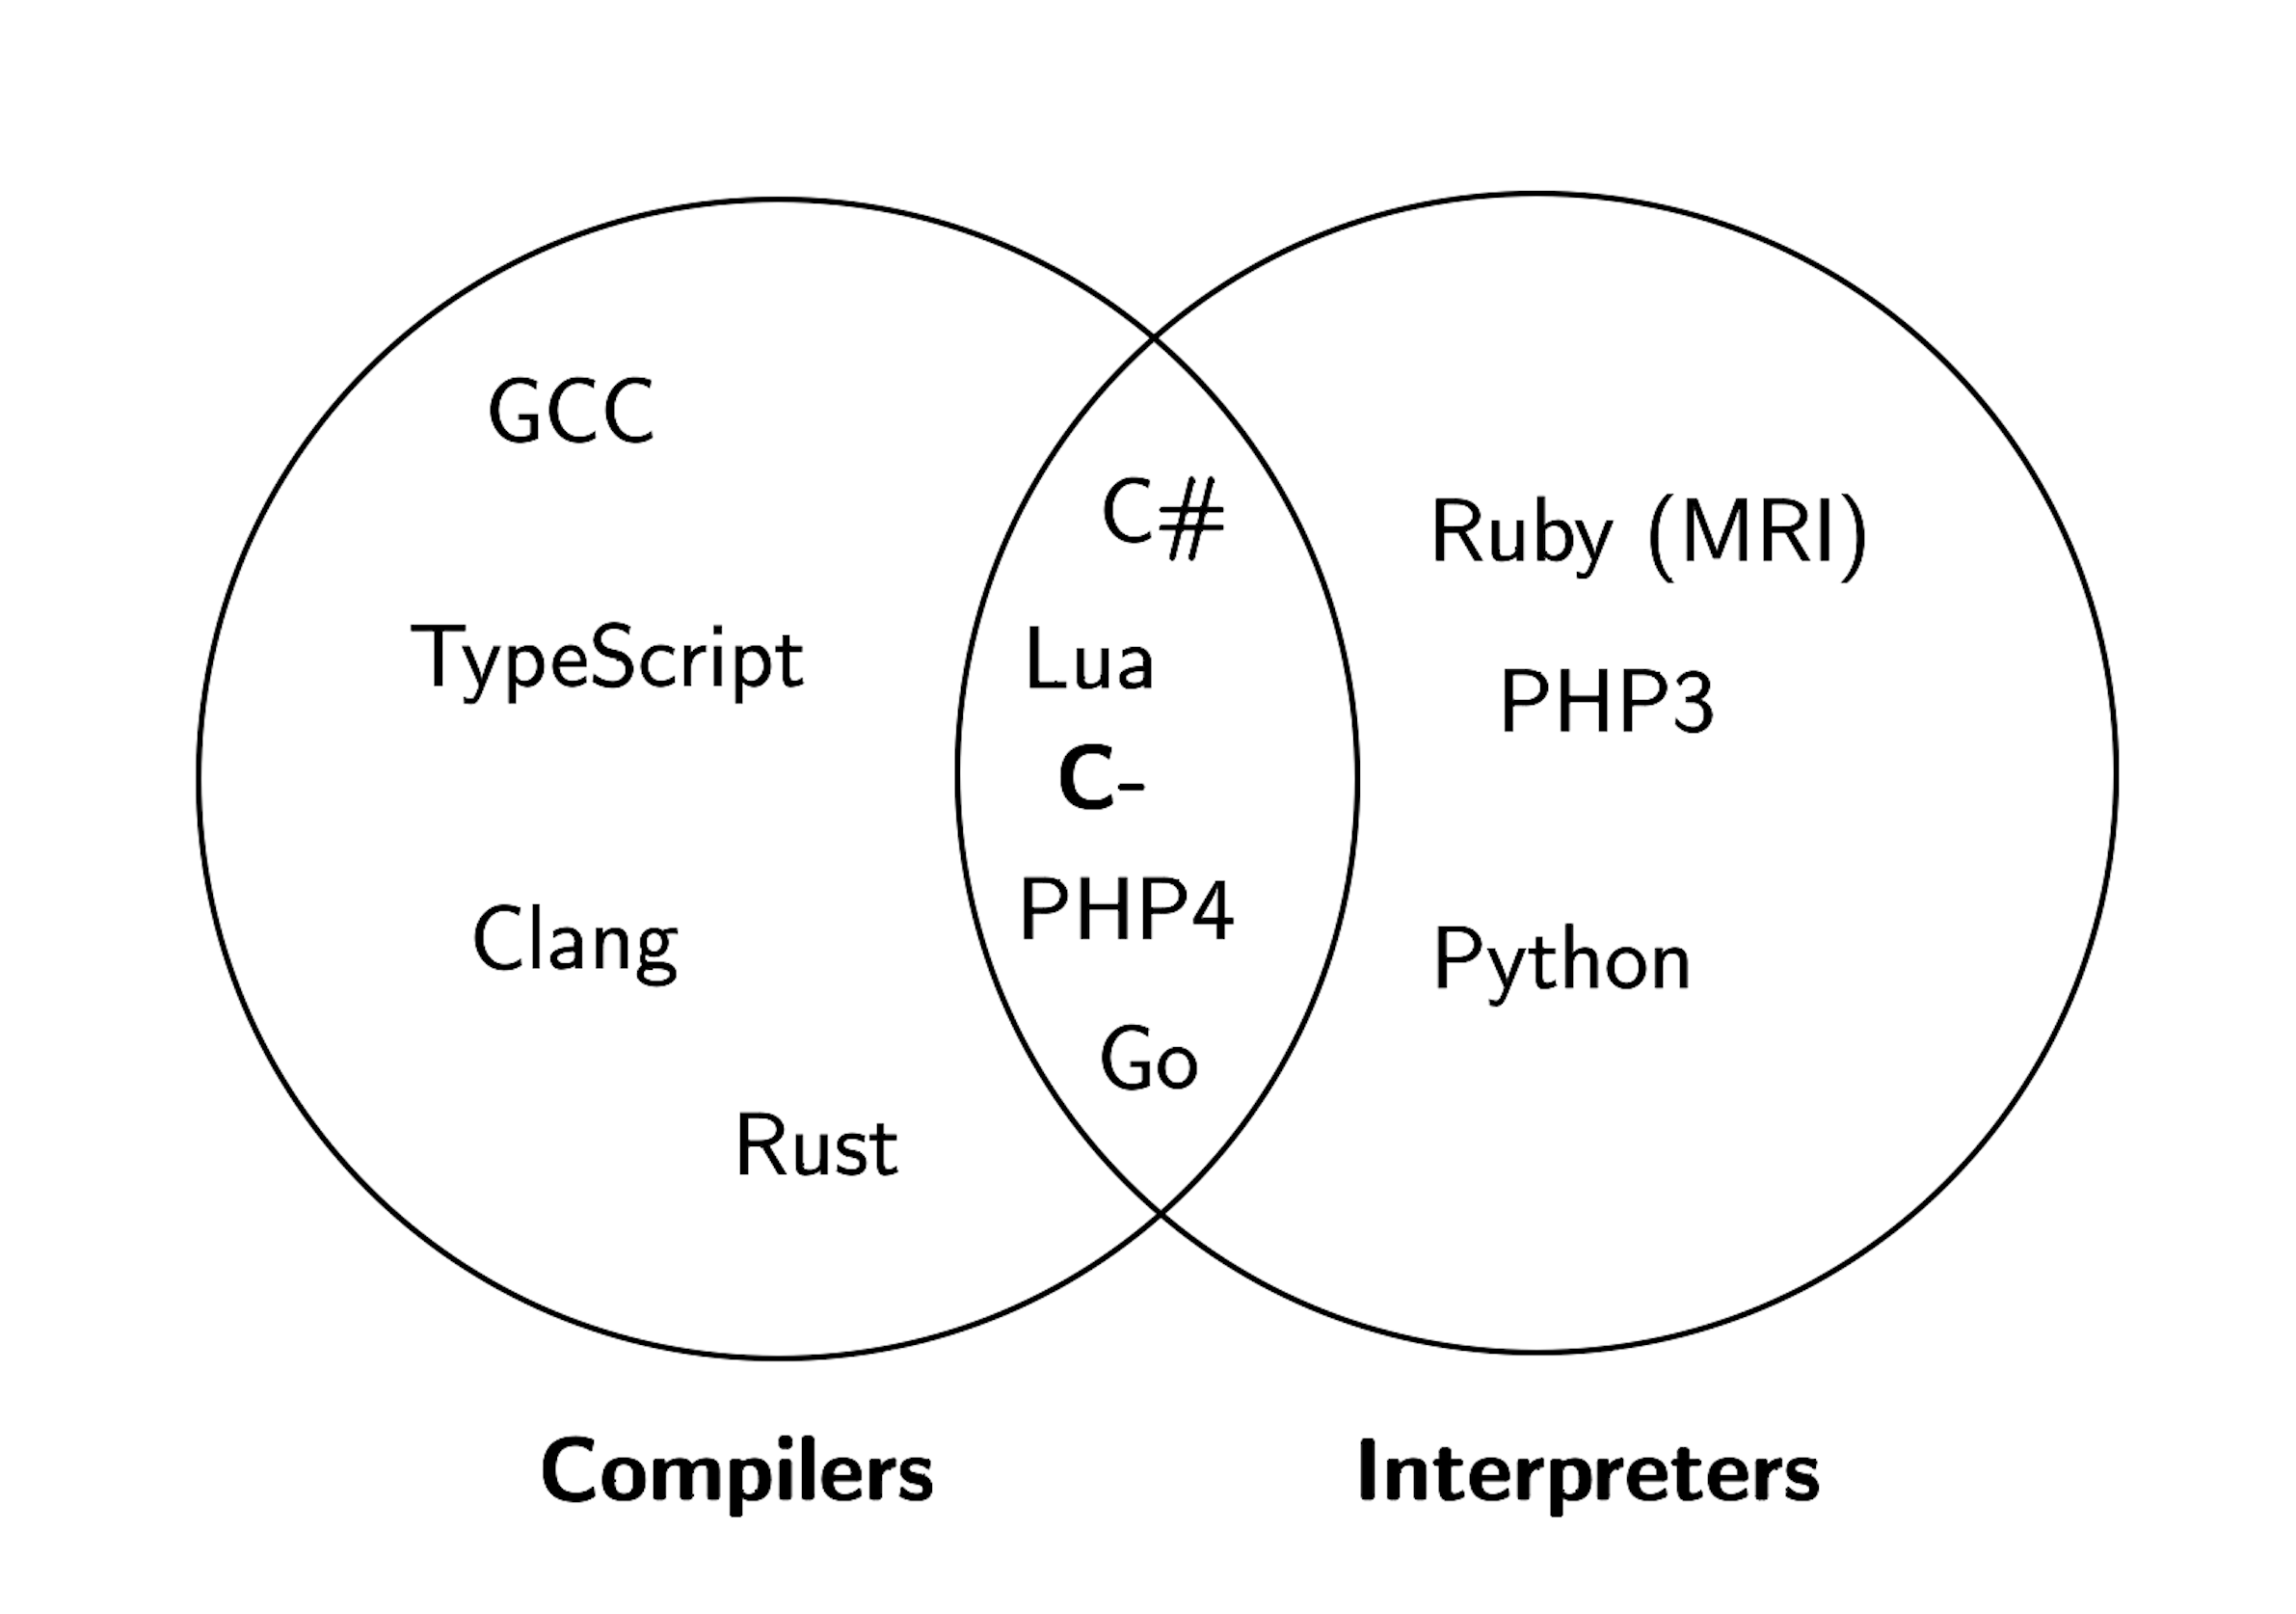
\includegraphics[width=0.75\textwidth]{gfx/venn.png}
\end{figure}

Our implementation, C-, lives in the middle area as it internally compiles to bytecode and then sends it to the \ac{VM}. 





%*****************************************
%*****************************************
%*****************************************
%*****************************************
%*****************************************





% !TEX root = classicthesis.tex

%*****************************************
\chapter{The C- Language}\label{ch:dashC}
%*****************************************
%\setcounter{figure}{10}
% \NoCaseChange{Homo Sapiens}

Although throughout the rest of this project we'll explore every nook and cranny of the C- languge, we spend this chapter to provide a small introduction to the general syntax, as a sort of preview of what our intepreter will use. We'll leave out many of the edge cases and details for later on and start with the mandatory \verb+"Hello, World!"+. 

\begin{lstlisting}[language=C]
print "Hello, world!";

// Prints Hello, world!
\end{lstlisting}

The \verb+//+ line comment and trailing semicolon at the end of the expression point towards C-like syntax, which is what C- derives from. Note that there are no parenthesis around the string because we plan to have \verb+print+ as a built-in statement rather than as a library function. 

\section{A Semantic Introduction}

\subsection{Dynamic Typing}

Unlike the language we are using to implement it, C- is dynamically typed, meaning that type is associated with run-time values rather than named variables, as type checking is done at run-time. We show a following example for one of the features that type checking provides. 

\begin{lstlisting}[language=C]
var a  = 1;
var b = "two";

print a + b;

// Returns a type error; we are trying to sum a string and integer
\end{lstlisting}

We choose this method of implementation because of it's ease compared to a statically typed language, and because we can implement features such as reflection (the ability for a process to examine or modify its own behaviour) or downcasting (casting a reference of a base class to one of its derived classes). In the context of C++, downcasting manually casts the base class's object to the derived class's object, meaning we must specify the explicit typecast. Furthermore, the derived class can now add new functionality such as new data members which could not apply to the base class. Let's illustrate an example in C++.

\begin{lstlisting}[language=C++]
class Parent  
{  
    public:  
        void base()  
        {  
            cout << "parent" << endl;   
        }  
};  
  
class Child : public Parent  
{  
    public:  
        void derive()  
        {  
            cout << "child" << endl;  
        }  
};  
  
int main ()  
{  
    Parent pobj; // create the Parent's object
    Child *cobj; // create the Child's object  
      
    // explicit type cast is required in downcasting  
    cobj = (Child *) &pobj;  
    cobj -> derive();  
      
    return 0;  
}  

// Outputs "child"
\end{lstlisting}

\subsection{Memory Management}

High level languages typically eliminate the tedious approach of freeing and allocating system memory (such as in C with \verb+free()+), which is the approach we will be taking with C-. There are two approaches to automatic memory management, reference counting and tracing garbage collection, also just known as garbage collection (\acs{GC}). Note that reference counters are method of ``garbage collection'' but tracing garbage collection are used so often that both terms are now synonymous.

Reference counters are a programming technique of storing the number of references, pointers, or handles to a resource, such as an object, a block of memory or disk space. These objects are reclaimed straight they can no longer referenced, unlike garbage collection, typically used in systems with limited memory to maintain responsiveness. Furthermore, it means non-memory resources such as operating system objects can be effectively managed, which are often much scarcer than memory. Most languages that started out using reference counters end up adding a full tracing garbage collecter, or at least enough of one to clean up object cycles. 

Tracing garbage collection consists of determining which objects should be deallocated (``garbage collected'') by tracing which objects are reachable by a chain of references from certain ``root'' objects, and considering the rest as ``garbage'' and collecting them. This approach is typically more difficult due to the need to work at the level of raw memory.

\subsection{Data Types}

In the C- programming language, built-in data types are the atomic bricks that store every item of a program, and we only need to employ a few.

Firstly, the boolean, a data type which has only two possible values, and a string literal to indicate each, unlike C which uses an unsigned integer. They are intended to signify true logical and mathematical or the negation of it, and we often see it used in conjunction with comparison operators. 

\begin{lstlisting}[language=C]
true; // not false
false; // not true
\end{lstlisting}

\subsection{Numbers}

Unlike C++, with number types such as \verb+int+, \verb+double+ and \verb+long long+, C- only utilizes a floating point double-precision (upto 15 decimal digits) number. This keeps things relatively simple while remaining relatively flexible and covering a wide range of numbers, only sacrificing a small amount of speed and memory. Furthermore, we will not implement hexadecimal or other number system bases, settling for only basic integer and decimal literals.

\begin{lstlisting}[language=C]
452;  // integer
923.00123; // floating point number
\end{lstlisting}

\subsection{Strings}

We've encountered this data type multiple times, even right from the beginning in our \verb+Hello, World!+ example. These are just a sequence of characters that store typically human-readable data, such as words or sentences and often uses character encoding, which will be one of the challenges to implement later on. 

\begin{lstlisting}[language=C]
"";  // empty string
"string"; // standard string
\end{lstlisting}

\subsection{Null}

Finally we have our final built in data type, \verb+null+, which is almost indentical to its C counterpart. The null pointer is used to indicate that the pointer does not refer to a valid object. Note that normally the null pointer is not the same as an unitialised pointer, but we will be using them as one. 

\section{Expressions and Statements}

If data types are the bricks to our C- city, expressions and statements would be our houses. We should make a distinction between statements, which are executed, and expressions, which are evaluated. Expressions always evaluate to a value, which statements do not. However, expressions are often used as part of a larger statement.

\subsection{Arithmetic}

These will be familiar and are just the standard basic arithmetic operations, including modulo.

\begin{lstlisting}[language=C]
183 + 298; // returns 481
901 - 873; // returns 28
81 * 12; // returns 972 
672 / 16; // returns 42
254 \% 32 // returns 30
\end{lstlisting}

We call the number's we are computing the operations upon, the operands and the ``\verb-+-, \verb+-+, \verb+*+, \verb+/+ or \verb+%+'' the operator. As we are performing this process with two operands, we call them binary operators. Futhermore, most of these are infix operators, except \verb+-+ which is both an prefix operator (when used for negation) and a infix operator (when used for subtraction). We also have postfix operators (which come before the operands) and misfix operators, which have more than two operands and the operators are interleaved between them. An example from C is the ``ternary'' operator, illustrated below:

\begin{lstlisting}[language=C]
condition ? thenArm : elseArm;
\end{lstlisting}

All these operators (except \verb-+-, which can be used to concatenate strings) only work on the \verb+number+ type and if any other type is fed through, a type error will be returned.

\subsection{Comparison and Equality}

We can make use of the \verb+boolean+ type by comparing \verb+number+ types using comparison operators. This is especially useful for iterating through loops for a set amount of time, such as if we wanted to print the first ten consecutive natural numbers. 

\begin{lstlisting}[language=C]
var a = 1;
while (a <= 10) {
  print a;
  a = a + 1;
}
\end{lstlisting}

We have four different comparison operators, listed below: 

\begin{lstlisting}[language=C]
2 < 3; // less than
2 <= 4; // less than or equal to
5 > 1; // greater than
19 >= 19; // greater than or equal to 
\end{lstlisting}

We can also use equality operators to test any two different types, any this also returns a \verb+boolean+ type. For example:

\begin{lstlisting}[language=C]
1 == 2 // returns false
"a" != "b" // returns true
\end{lstlisting}

Note that values of different types can be compared late, and can never be equivalent: 

\begin{lstlisting}[language=C]
1 == "one"; // returns false
\end{lstlisting}

Equality is also often used to test if an element already exists in a set, or to access to a value through a key.

\subsection{Logical Operators}

In logic, a logical operator is a logical constant which is used to connect logical formulas. Common operators include negation, disjunction, conjuction, implication and equivalence, and are interpreted as truth functions. Logical operators can be used to link zero or more statements, so one can speak about \(n\)-ary logical operators. Note that the \verb+boolean+ types, \verb+True+ and \verb+False+ are known as zero-ary operators, while negation is known as a one-ary operator, and so on. 

Outside the field of computer science, where we denote this with symbols such as \verb+AND+ and \verb+NOT+, these symbols are represneted non-ambigiously with special symbols. We list them down below. 

\begin{itemize}

\item Negation (\verb+NOT+) – This is an operation that is intuitively interpreted as true when some proposition \(P\) is false, or not true, and false when some proposition \(P\) is false. We can denote this in formal logic as ¬\(P\) (the most common notation), \(\sim P\) or \(NP\). This is similar to how in mathematical set theory \(\setminus \) is used to indicate `not in the set of' (i.e \({\displaystyle U\setminus A}\) is the set of all members of \(U\) that are not members of \(A\)). The truth table is as follows:


\begin{table}[h]
{\centering
\begin{tabular}{|c|c|}
\hline
\rowcolor[HTML]{EFEFEF} 
\(P\) & \(\neg P\) \\ \hline
True       & False           \\ \hline
False      & True            \\ \hline
\end{tabular} \par }
\end{table}

We will use the \verb+!+ character as a prefix to denote \verb+NOT+. 

\begin{lstlisting}[language=C]
!true; // returns false
!false; // returns true
\end{lstlisting}

\item Conjunction (\verb+AND+) – This is an operator that takes two operands, say \(A\) and \(B\) and is only true when some both are true. We denote this We most often notate this as \(\wedge\) and can define it in terms of the \verb+NOT+ and \verb+OR+ functions as  \(A \wedge B = \neg(\neg A \lor \neg B) \). Below is the truth table for the \verb+AND+ operator:

\begin{table}[h]
{\centering
\begin{tabular}{|c|c|c|}
\hline
\rowcolor[HTML]{EFEFEF} 
\(A\)                           & \(B\)                 & \(A \wedge B\) \\ \hline
True                        & True                       & True       \\ \hline
True                        & False                      & False      \\ \hline
\multicolumn{1}{|l|}{False} & \multicolumn{1}{l|}{True}  & False      \\ \hline
\multicolumn{1}{|l|}{False} & \multicolumn{1}{l|}{False} & False      \\ \hline
\end{tabular} \par }
\end{table}

In C-, we'll just denote this with \verb+and+.

\begin{lstlisting}[language=C]
true and false; // returns false
true and true;  // returns true
\end{lstlisting} 

\item Disjuntion (\verb+OR+) – This is an operator that returns \verb+True+ if either of its operands \(A\) or \(B\) are true and \verb+False+ if both \(A\) and \(B\) are false. This is typically denoted with \(\vee\) and we can define it in terms of other operators as \(A \vee B =  \neg ((\neg A) \wedge (\neg B))\). Below is the truth table:

\begin{table}[h]
{\centering
\begin{tabular}{|c|c|c|}
\hline
\rowcolor[HTML]{EFEFEF} 
\(A\)                       & \(B\)                      & \(A \vee B\) \\ \hline
True                        & True                       & True         \\ \hline
True                        & False                      & True         \\ \hline
\multicolumn{1}{|l|}{False} & \multicolumn{1}{l|}{True}  & True         \\ \hline
\multicolumn{1}{|l|}{False} & \multicolumn{1}{l|}{False} & False        \\ \hline
\end{tabular} \par }
\end{table}

In C-, we'll again just denote this with the word \verb+or+.

\begin{lstlisting}[language=C]
false or true;  // returns true
false or false; // returns false.
\end{lstlisting} 
\end{itemize}

In C-, and programming langauges in general \verb+and+ and \verb+or+ are more like control flow structures rather than an operator. For example, if the left operand of a \verb\or\ statement is true, the right statement is skipped, effectively causing a short circuit. 

From an overview we can say that all these operations have the same associativity and precedence as in C, and that this order can be modifified with \verb+()+

\subsection{Statements}

Recall that statements do not evaluate to a value, unlike expressions, and instead aim to produce and effect, say by modifying a state, reading input or producing output. Again, if we go back to our \verb+Hello, World!+ example, we have created a statement as \verb+print+ evalues a single expression and displays the result. 

\begin{lstlisting}[language=C]
print "Hello, world!";
\end{lstlisting}

An expression followed by a semicolon (\verb+;+) promotes the expression to an expression statement. Furthermore, we can wrap multiple statements into where only one is expected using a block, which affects scoping. 

\begin{lstlisting}[language=C]
{
  print "a";
  print "b";
}
\end{lstlisting}

\section{Variables, Loops and Functions}

\subsection{Variables}

We can declare variables using \verb+var+ statements, meaning we do not usually have to specify the type. If we don't include the initializer statement, the variable’s value defaults to \verb+nil+.

\begin{lstlisting}[language=C]
var a = "a"; // stores the string "a"
var b; // stores the nil type
\end{lstlisting}

We can then access and remodify variables by calling on it's name.

\begin{lstlisting}[language=C]
var a = "b"; 
print b; // returns "b"
\end{lstlisting}

\subsection{Loops}

Loops are essential for the control flow of a program, meaning we can skip code to execute blocks of code multiple times. Although we could make use of our logical connectives \verb+and+, \verb+not+ and \verb+or+ for branching and recursion techniques for iterating through code, we feel it would be more convinient to add simple looping statements into C-. 

We include three statements from the C language, starting with \verb+if+. When our interpreter finds an \verb+if+ statement, it expects a \verb+boolean+ condition, and evalues that condition. If the condition is true, then the following statements are executed, while if it is false, the nested block is skipped and the code (possibly within an \verb+else+ statement) after is executed.

\begin{lstlisting}[language=C]
if (condition) {
  print "a";
} else {
  print "b";
}
\end{lstlisting}

We can think of our next statement, the \verb+while+ loop as a set of repeated \verb+if+ statements, a control flow statement that allows code to be repeatedly executed based on some \verb+boolean+ condition. We return to our example of printing the first ten natural numbers

\begin{lstlisting}[language=C]
var a = 1;
while (a <= 10) {
  print a;
  a = a + 1;
}
\end{lstlisting}

We have decided to omit the \verb+do while+ statement, as it is similar enough to the \verb+while+ statement.
Finally we have \verb+for+ loops, which are used mainly for iteration; running a section of code repeatedly until some condition is satisfied. Let's rewrite our code for printing the first ten natural numbers using a \verb+for+ loop.

\begin{lstlisting}[language=C]
for (var a = 1; a < 10; a = a + 1) {
  print a;
}
\end{lstlisting}

Some languages ikmplement a \verb+for-in+ or \verb+foreach+ loops for explicitly iterating over various sequence types, which can be handy, but we'll stick with C's standard \verb+for+ loop. 

\subsection{Functions}

We carry over the same syntax from C for calling functions: 

\begin{lstlisting}[language=C]
function(a, b);
\end{lstlisting}

Note that we can abstain from passing any parameters to the function, which still calls upon it, but we still need the empty parenthesis otherwise we just refer to the function. 

Declaring functions can be done with \verb+fun+, similar to \verb+var+. Recall that a declaration binds the function’s type to its name so that calls can be type-checked but does not provide a body. A definition declares the function and also fills in the body so that the function can be compiled. This distinction is not very meaningful in C- because it is dynamically typed. 

Although these terms are used interchangeably, we also clarify the difference between a parameter and argument. A parameter is a variable that holds the value of the argument inside the body of the function, while an argument is an actual value you pass to a function when you call it.

\begin{lstlisting}[language=C]
fun sum(a, b) {
  return a + b;
}
\end{lstlisting}

Note that a function body is always a block, and that a function always has to return a value, otherwise it just implicitly returns a value of the \verb+nil+ type. We can call multiple functions below, as shown below:

\begin{lstlisting}[language=python]
fun identity(a) {
  return a;
}

print identity(sum)(a, b);
\end{lstlisting}

We can also declare functions within other functions:


\begin{lstlisting}[language=C]
fun global() {
  fun local() {
    return "a";
  }

  local();
}
\end{lstlisting}

Here, \verb+local()+ accesses a local variable declared outside of its body in the surrounding function, which works by \verb+local()+ holding on to references to any surrounding variables that it uses so that they stay around even after the outer function has returned. Functions, such as \verb+local()+, that do this are known as closures.

\section{Classes}

Classes are a key feature of \ac{OOP}, a programming paradigm based on the concept of objects, which contain data and code. This data is stored as fields (which is known as attributes or properties), and the code is in the form of procedures (known as methods). 

Although most languages using \ac{OOP} such as C++, C\# and Java uses classes, we also have another possible type of objects; prototypes.

In regular class-based languages, the two main ideas are classes (extensible templates for creating objects) and instances (concrete occurences of any object). Classes contain the methods and inheritance chain. To call a method on an instance, there is always a level of indirection, meaning you have look up the instance’s class and then you find the method there.

Prototype-based languages merge these two concepts. There are only objects—no classes—and each individual object may contain state and methods. Objects can directly inherit (known as delegate in prototype-based languages) from each other, meaning that prototypal languages are more fundamental than classes. This also makes them a lot easier and quicker to implement and have a lot more options for abstract and unusual data patterns. 

However, we find that often programming languages utilizing prototypes are less comfortable to the average user, which is an important factor for desigining C-.

We can declare a class and it's methods as follows:

\begin{lstlisting}[language=python]
class a {
  b() {
    print "c";
  }

  d(e) {
    print "f" + e;
  }
}
\end{lstlisting}

The body of a class contains its methods, which are declared like functions, but without the keyword. When the class declaration is executed, C- creates a class object and stores that in a variable named after the class. To keep things simple in C-, the class itself is a factory function for instances: 

\begin{lstlisting}[language=C++]
var a = b();
print b; // returns the b instance
\end{lstlisting}

Classes aren't very useful by themselves, and we need to implement some sort of method to encapsulate behvaiour and state together, which can be done using the notion of fields. Like other dynamically typed languages, C- lets us freely add properties onto objects. 

If we want to access a field or method on the current object from within a method we can use the \verb+this+ statement. Note that assigning to a field creates it if it doesn't already exist.

\begin{lstlisting}[language=ruby]
class a {
  init(b, c) {
    this.b = b;
    this.c = c;
  }
}

var d = a("e", "f");
d.g("h");
\end{lstlisting}

Part of encapsulating data within an object is ensuring the object is in a valid state when it’s created, which can be done by defining an initializer, \verb+init()+. Any parameters passed to the class are forwarded to its initializer and it is called automatically when the object is constructed.

C- supports single inheritance, which can be declared by using a less-than (\verb+<+). 

\begin{lstlisting}[language=ruby]
class a < b {
  ;
}
\end{lstlisting}

Here \verb+a+ is the derived class (also known as the subclass) while \verb+b+ is the base class (also known as the superclass). Every method defined in the superclass, even \verb+init()+, is also available to its subclasses. To call a method on our own instance without hitting our own methods can be done with \verb+super+.

In a true OOP language every object is an instance of a class, even primitive values like numbers and Booleans, but in C- we aim to keep the feature set relativelt minimal.

\section{The Standard Library}

This is the last section in the overview, the standard library, whcih is the core set of instructions and functionality we directly implement in the interpreter and that all user-defined behavior is built on top of.

We've already seen the \verb+print+ function which can be used to output data to the user, and we'll need a function which can be used to record the amount of time a program takes to be able to compare different optimizations, so we use \verb+clock+ which returns the number of seconds since the program started. Other utility functions include:

\begin{itemize}
 \item \verb+exit(x)+ – exits the process with the number \verb+x+ as the exit code. \verb+x+ must be a whole number between 0 and 255 inclusive.
 \item \verb+str(x)+ – converts the value \verb+x+ into a string.
 \item \verb+type(x)+ – returns the type of the value \verb+x+ as a string.
 \item \verb+eprint(x)+ – prints the value v to the standard error stream
 \item \verb+argc()+ – returns the number of command line arguments the interpreter was launched with.
 \item \verb+argv(i)+ – returns the command line argument at position \verb+i+; zero should be the interpreter program, and numbers up to (but not including) the return value of \verb+argc()+ are additional arguments.
 \item \verb+chr(x)+ – returns a one-character string whose first byte is the number represented by \verb+x+. The valid range for \verb+x+ depends on how the platform treats C's char type; for signed char it can be any whole number between -128 and 127 inclusive.
\end{itemize}

We also add some basic mathematical functions:

\begin{itemize}
 \item \verb+ceil(x)+ \( \lceil x \rceil \) – returns the number \verb+x+ rounded up to the nearest whole number. For example, 0.4 would be rounded to 1. 
 \item \verb+floor(x)+ \( \lfloor x \rfloor \) – returns the number \verb+x+ rounded down to the nearest whole number. For example, 1.9 would be rounded to 1.
 \item \verb+round(x)+ – returns the number \verb+x+ rounded to the nearest whole number. For example, 1.4 would be rounded to 1 and 1.6 would be rounded to 2.  
\end{itemize}

We plan to add trigonometric functions such as \verb+sin(x)+ as an extenstion to the project.

%*****************************************
%*****************************************
%*****************************************
%*****************************************
%*****************************************

\part{Analysis}
% !TEX root = classicthesis.tex

%************************************************
\chapter{A Bytecode Implementation}\label{ch:bytecode} % $\mathbb{ZNR}$
%************************************************

\section{Why not AST?}

We choose a bytecode implementation for it's speed compared to the main rival candidate for an interpreter; a tree-walk interpreter. We've explained the general reason for this in our design overview. 

In more depth, when we write any piece of code that's to be compiled using an AST, it's just not memory efficient. Each fragment of code becomes an AST node. Take the expression \verb%1 + 2% turns into a flurry of objects with pointers, each adding an extra 32 or 64 bits of overhead to the object. Not only this, when spreading our data across the heap in a loosely connected web of objects, we have problems with spatial locality. 

Spatial locality (also known as data locality) refers to the use of data elements within relatively close storage locations. Modern CPUs can process data much faster than they can retreive it from RAM, leading to the use of (multiple layers of) caching. If a piece of memory it needs is already in the cache, it can be loaded more quickly, even upto two orders of magnitude faster. 

The CPU ``predicts'' what data we need by pulling in adjacent bytes to what is currently being read from RAM and stores them in cache. If our program next requests some data close enough to be inside that cache line, we end up with a faster program experience. To take advantage of this, the way we represent code in memory should be dense and ordered like it’s read. 

However, when using an AST, the sub-objects can be stored anyway. Every step the tree-walker takes where it follows a reference to a child node may step outside the bounds of the cache and force the CPU to stall until the next data can be recalled from RAM\@. Just the overhead of the tree nodes with all of their pointer fields and object headers tends to push objects away from each other and out of the cache.

\section{Why Bytecode?}

Let's consider the other end of the speed spectrum first, compiling to native machine code. Compiling directly to the native instruction set the chip supports is what the fastest languages do, where the CPU cranks through the instructions, decoding and executing each one in order. There is no tree structure like our AST, and control flow is handled by jumping from one point in the code directly to another. This comes at a cost, as firstly this comilation process is not easy, especially with newer chips which more complicated architectures. Furthermore, there is no portability, as we'd only be producing for one architecture type of the multiple that are used today. To get our language on all of them, we'd need to learn all of their instruction sets and write a separate back end for each one.

Bytecode is in the middle of both extremes of these implementations, retaining the portability of a tree-walker and sacrifices some simplicity for an increase in performance. Although bytecode resembles machine code in it's dense, linear sequence of binary instructions, simpler, higher-level instruction set than any real chip. This keeps the overhead low, and takes advantage of the caching feature of a chip. 

It's essentially like writing for an idealised fantasy instruction set for some perfect architecture. However, obviously when we develop for such an architecture that doesn't exist, we can't actually run it normally. This means we need to write an emulator – a simulated chip written in software that interprets the bytecode one instruction at a time and simulates what the perfect architecture would do. This is known as a \ac{VM}.

This does add overhead, which is why using a bytecode implementation is not as fast as writing native machine code, but in return we receive portability to run on basically any hardware we want. Below we outline our implementation process, although we probably won't build each phase in order.


\begin{figure}[h]
\centering
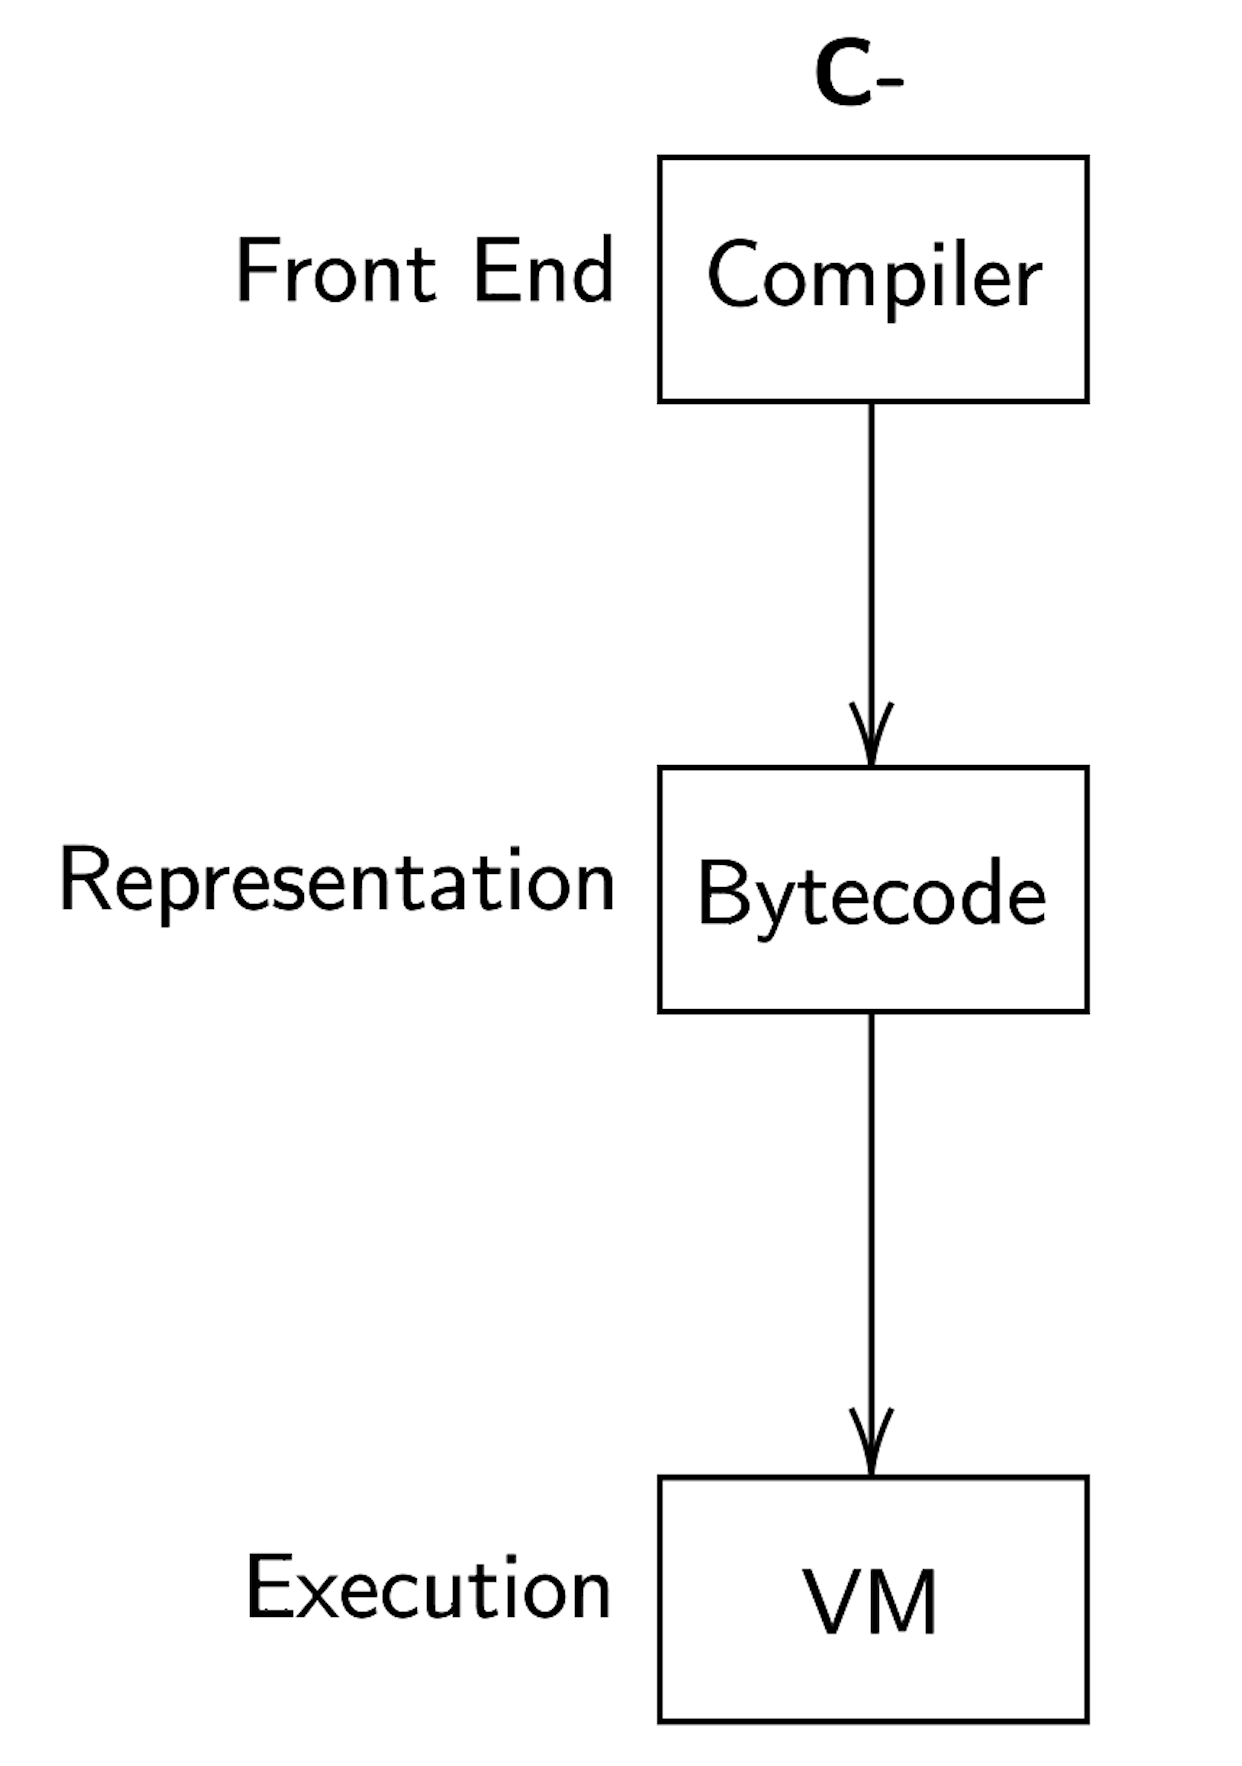
\includegraphics[width=0.35\textwidth]{gfx/process.png}
\caption{Implementation Process}
\end{figure}

\section{Laying the Foundation}

We'll start with our \verb+main()+ function in \verb+main.c+. For now we'll just create an empty function.

\begin{lstlisting}[language=C]
// main.c

#include "common.h"

int main(int argc, const char* argv[]) {
  return 0;
}
\end{lstlisting}

As we can see by the quotation marks, the \verb+common.h+ file is not part of the C standard library. Let's create it now:

\begin{lstlisting}[language=C]
// common.h

#ifndef common_h
#define common_h

#include <stdbool.h>
#include <stddef.h>
#include <stdint.h>

#endif
\end{lstlisting}

This is where we store the additional C types we'll use throughout the process. For now, we've added \verb+NULL+, the C99 \verb+bool+ data type which macros true and false expand to \verb.1. and \verb.0. respectively, and some more specific types of integers such as \verb+uint8_t+ (unsigned integers). 

In \emph{Crafting Interpreters}, Bob Nystrom refers to chunks as sequences of bytecode, so we draw from that to create the module \verb+chunk.h+. In bytecode, each instruction has a one-byte opcode (operation code), which controls what kind of instruction we're dealing with. We define that here. 

\begin{lstlisting}[language=C]
// chunk.h

#ifndef chunk_h
#define chunk_h

#include "common.h"

typedef enum {
  OP_RETURN,
} OpCode;

#endif
\end{lstlisting}

The only instruction \verb+OP_RETURN+, will eventually mean ``return from the currrent function'', but has no use at the moment. 


\subsection{Dynamic Arrays}

Let's now create the \verb+struct+ to hold the data that will be stored alongside the instructions.

\begin{lstlisting}[language=C]
// chunk.h

typedef struct {
  uint8_t* code;
} Chunk;
\end{lstlisting}

This just creates a wrapper arround an area of bytes, however because we don't know how big the array of data needs to be before compiling a chunk we need, it needs to be dynamic. Implementing this is simple, we just need to declare an additional two quantities: the number of elements in the array we have allocated (\verb+capacity+) and how many of these are in use (\verb+count+).

\begin{lstlisting}[language=C]
// chunk.h

typedef struct {
  int count;
  int capacity;
  uint8_t* code;
} Chunk;
\end{lstlisting}

If \verb+count+ is less than \verb.capacity. then adding an element is as simple as allocating the new element to the free space and incrementing count. If there is no spare capacity then our process is as follows: 

\begin{itemize}
 \item Allocate a new array with more capacity and carry over the existing elements from the old array to the new one. 
 \item Store the new capacity and delete the old array
 \item Update \verb+code+ to point to the new array and store the element in the new array
 \item Increment \verb+count+
\end{itemize}

Note that through the use of amortized analysis, we can see that as long as we grow the array by a multiple of its current size, when we average out the cost of a sequence of appends, each append only takes \(\mathcal{O}(1)\).

Now that our \verb.struct. is ready, we can implement the functions to work with it. Because C doesn't have constructors, we need to declare a function to initialize a new chunk.

\begin{lstlisting}[language=C]
// chunk.h

void initChunk(Chunk* chunk);
\end{lstlisting}

Let's implement it by creating a new file, \verb+chunk.c+:

\begin{lstlisting}[language=C]
// chunk.c

#include <stdlib.h>

#include "chunk.h"

void initChunk(Chunk* chunk) {
  chunk->count = 0;
  chunk->capacity = 0;
  chunk->code = NULL;
}
\end{lstlisting}

Note that we don't even allocate a raw array to our dynamic array; it starts of completely empty. Let's create a new function to append a byte to the end of a chunk:

\begin{lstlisting}[language=C]
// chunk.c

void writeChunk(Chunk* chunk, uint8_t byte) {
  if (chunk->capacity < chunk->count + 1) {
    int oldCapacity = chunk->capacity;
    chunk->capacity = GROW_CAPACITY(oldCapacity);
    chunk->code = GROW_ARRAY(uint8_t, chunk->code,
        oldCapacity, chunk->capacity);
  }

  chunk->code[chunk->count] = byte;
  chunk->count++;
}\end{lstlisting}

The first thing that we need to do is see if the current array already has the capacity for the new byte, and if it doesn't we grow the array to make room. This will happen every time on the  first write, as we've set the original \verb+capacity+ to \verb.0.. 

To increase the array's size, we first calculate the new capacity and then adjust the array to match it. These lower-level memory operations are now defined in a new module \verb+memory.h+.

\begin{lstlisting}[language=C]
// memory.h

#ifndef memory_h
#define memory_h

#include "common.h"

#define GROW_CAPACITY(capacity) \
    ((capacity) < 8 ? 8 : (capacity) * 2)

#endif
\end{lstlisting}

Since we're using it in the process of chunks, we should also include it in \verb+chunk.c+ using:

\begin{lstlisting}[language=C]
// chunk.c

#include "memory.h"
\end{lstlisting}

This macro calculates a new capacity based on the current capacity, and for optimal performance, it scales relative to the previous size. Typically, we increase it by a factor of two, although 1.5× is another common choice.

We've also accounted for cases where the current capacity is zero. In such instances, we start with eight elements instead of one, reducing unnecessary memory overhead for very small arrays, albeit at the cost of some wasted space. The choice of the number eight was somewhat arbitrary in this context, as most dynamic array implementations have a similar minimum threshold. 

Once the desired capacity is determined, we proceed to create or expand the array to match that size using the \verb+GROW_ARRAY()+ function.

\begin{lstlisting}[language=C]
// memory.h

#define GROW_ARRAY(type, pointer, oldCount, newCount) \
    (type*)reallocate(pointer, sizeof(type) * (oldCount), \
        sizeof(type) * (newCount))

void* reallocate(void* pointer, size_t oldSize, size_t newSize);
\end{lstlisting}

This macro simplifies a function call to \verb.reallocate(). where the primary work is accomplished. It takes care of determining the size of the array's element type and performing the necessary casting to ensure the resulting \verb+void*+ is of the correct type.

The \verb.reallocate(). function serves as the central function for all dynamic memory management within C-. It handles various tasks such as memory allocation, deallocation, and resizing existing allocations. This consolidation of memory operations into a single function becomes crucial later when we introduce a garbage collector responsible for monitoring memory usage.

The two size arguments provided to \verb.reallocate(). dictate the specific operation to be executed:


\begin{table}[h]
{\centering
\begin{tabular}{|c|c|c|}
\hline
\rowcolor[HTML]{EFEFEF} 
\verb.oldSize. & \verb.newSize.              & Operation                  \\ \hline
0              & Non-zero                    & Allocate new block         \\ \hline
Non-zero       & 0                           & Free allocation            \\ \hline
Non-zero       & Smaller than \verb.oldSize. & Shrink existing allocation \\ \hline
Non-zero       & Larger than \verb.oldSize.  & Grow existing allocation   \\ \hline
\end{tabular} \par}
\end{table}

Although this looks like a lot of different cases to consider for, the implementation is quite simple. We'll add this to a new file \verb,memory.c,

\begin{lstlisting}[language=C]
// memory.c

#include <stdlib.h>

#include "memory.h"

void* reallocate(void* pointer, size_t oldSize, size_t newSize) {
  if (newSize == 0) {
    free(pointer);
    return NULL;
  }

  void* result = realloc(pointer, newSize);
  return result;
}
\end{lstlisting}

When \verb.newSize. is zero, we handle deallocation ourselves by calling \verb,free(),. Otherwise, we rely on the C standard library's \verb.realloc(). function, which conveniently supports the other three aspects of our memory management policy.

The interesting cases arise when both \verb.oldSize. and \verb.newSize. are non-zero. In such instances, \verb.realloc(). is instructed to resize the previously allocated memory block. If the new size is smaller than the existing block, it updates the block's size and returns the same pointer provided.

If the new size is larger, it attempts to expand the existing block, but this is contingent on there being available memory space beyond it. It can only do this if the memory following the block is not already in use. If there isn't enough room to grow the block, \verb.realloc(). takes an alternative approach: it allocates a new memory block of the desired size, copies the old data into it, frees the old block, and then returns a pointer to the new block.

This behavior aligns perfectly with our dynamic array requirements. However, it's crucial to acknowledge that due to the finite nature of computer resources, allocation can fail if there's insufficient memory. In such cases, \verb.realloc(). will return \verb.NULL., meaning we should add an extra fallback for this case:

\begin{lstlisting}[language=C]
// memory.c

void* result = realloc(pointer, newSize);
  if (result == NULL) exit(1);
  return result;
\end{lstlisting}

We still can't do anything very useful with the \ac{VM} without it getting it the memory it needs, but at least we can detect that  and abort the process instead of just returning a \verb/NULL/ pointer and it causing problems later.

Now we've found a way to create new chunks and write instructions to them. Because we're creating this in C, memory management is important and we need to find a way to free chunks as well. We declare it first:

\begin{lstlisting}[language=C]
// memory.h

void freeChunk(Chunk* chunk);
\end{lstlisting}

And implement it like so:

\begin{lstlisting}[language=C]
// memory.c

void freeChunk(Chunk* chunk) {
  FREE_ARRAY(uint8_t, chunk->code, chunk->capacity);
  initChunk(chunk);
}
\end{lstlisting}

This works by deallocating all the memory and then calling \verb/initChunk()/ to zero out the fields leaving the chunk in a (well defined) empty space. To free the memory completely, we need to add another macro to the header file.

\begin{lstlisting}[language=C]
// memory.h

#define FREE_ARRAY(type, pointer, oldCount) \
    reallocate(pointer, sizeof(type) * (oldCount), 0)
\end{lstlisting}

Like the other macro, \verb>GROW_ARRAY()>, this is a wrapper around a \verb.reallocate(). call which frees the memory by passing in zero for the new size.

\subsection{Disassembling Chunks}

Let's try our work by trying to hand-building a sample chunk. We'll test it through \verb,main.c,. 

\begin{lstlisting}[language=C]
// main.c

#include "common.h"
#include "chunk.h"

int main(int argc, const char* argv[]) {
  Chunk chunk;
  initChunk(&chunk);
  writeChunk(&chunk, OP_RETURN);
  freeChunk(&chunk);
  return 0;
\end{lstlisting}

We can run this and it doesn't return any errors, but we can't exactly confirm if our tests worked. This makes sense since all we've done it shift around bytes in memory and there's no human friendly way to see what we've created. To resolve this we're going to create a disassembler.

An assembler, in its traditional form, is a program designed to process a file containing human-readable mnemonic names for CPU instructions, such as \verb.ADD. and \verb.MULT., and convert them into their corresponding binary machine code representations. Conversely, a disassembler performs the reverse operation: when provided with a chunk of machine code, it generates a textual listing of the instructions contained within.

Let's pass the chunk in \verb,main.c, through the disassembler after creation:

\begin{lstlisting}[language=C]
// main.c

disassembleChunk(&chunk, "test chunk");
\end{lstlisting}

We should create a debug header for this as well:

\begin{lstlisting}[language=C]
// debug.h

#ifndef debug_h
#define debug_h

#include "chunk.h"

void disassembleChunk(Chunk* chunk, const char* name);
int disassembleInstruction(Chunk* chunk, int offset);

#endif
\end{lstlisting}

In the \verb.main(). function, we use \verb.disassembleChunk(). to disassemble all instructions in the chunk. This relies on another function that handles disassembling individual instructions. We've put this in the header file because we'll need to call upon it in later chapters as part of the \ac{VM}.

We should now implement this \verb.disassembleChunk(). function into a new file, \verb,debug.c,:

\begin{lstlisting}[language=C]
// debug.c

#include <stdio.h>

#include "debug.h"

void disassembleChunk(Chunk* chunk, const char* name) {
  printf("== %s ==\n", name);

  for (int offset = 0; offset < chunk->count;) {
    offset = disassembleInstruction(chunk, offset);
  }
}
\end{lstlisting}




%*****************************************
%*****************************************
%*****************************************
%*****************************************
%*****************************************

%\addtocontents{toc}{\protect\clearpage} % <--- just debug stuff, ignore
%\include{multiToC} % <--- just debug stuff, ignore for your documents
% ********************************************************************
% Backmatter
%*******************************************************
% \appendix
% %\renewcommand{\thechapter}{\alph{chapter}}
% \cleardoublepage
% \part{Appendix}
% %********************************************************************
% Appendix
%*******************************************************
% If problems with the headers: get headings in appendix etc. right
%\markboth{\spacedlowsmallcaps{Appendix}}{\spacedlowsmallcaps{Appendix}}
\chapter{Appendix Test}
Lorem ipsum at nusquam appellantur his, ut eos erant homero
concludaturque. Albucius appellantur deterruisset id eam, vivendum
partiendo dissentiet ei ius. Vis melius facilisis ea, sea id convenire
referrentur, takimata adolescens ex duo. Ei harum argumentum per. Eam
vidit exerci appetere ad, ut vel zzril intellegam interpretaris.
\graffito{More dummy text.}

%Errem omnium ea per, pro congue populo ornatus cu, ex qui dicant
%nemore melius. No pri diam iriure euismod. Graecis eleifend
%appellantur quo id. Id corpora inimicus nam, facer nonummy ne pro,
%kasd repudiandae ei mei. Mea menandri mediocrem dissentiet cu, ex
%nominati imperdiet nec, sea odio duis vocent ei. Tempor everti
%appareat cu ius, ridens audiam an qui, aliquid admodum conceptam ne
%qui. Vis ea melius nostrum, mel alienum euripidis eu.

\section{Appendix Section Test}
Test: \autoref{tab:moreexample} (This reference should have a 
lowercase, small caps \spacedlowsmallcaps{A} if the option 
\texttt{floatperchapter} is activated, just as in the table itself
 $\rightarrow$ however, this does not work at the moment.)

\begin{table}[h]
    \myfloatalign
  \begin{tabularx}{\textwidth}{Xll} \toprule
    \tableheadline{labitur bonorum pri no} & \tableheadline{que vista}
    & \tableheadline{human} \\ \midrule
    fastidii ea ius & germano &  demonstratea \\
    suscipit instructior & titulo & personas \\
    %postulant quo & westeuropee & sanctificatec \\
    \midrule
    quaestio philosophia & facto & demonstrated \\
    %autem vulputate ex & parola & romanic \\
    %usu mucius iisque & studio & sanctificatef \\
    \bottomrule
  \end{tabularx}
  \caption[Autem usu id]{Autem usu id.}
  \label{tab:moreexample}
\end{table}

%Nulla fastidii ea ius, exerci suscipit instructior te nam, in ullum
%postulant quo. Congue quaestio philosophia his at, sea odio autem
%vulputate ex. Cu usu mucius iisque voluptua. Sit maiorum propriae at,
%ea cum primis intellegat. Hinc cotidieque reprehendunt eu nec. Autem
%timeam deleniti usu id, in nec nibh altera.




\section{Another Appendix Section Test}
Equidem detraxit cu nam, vix eu delenit periculis. Eos ut vero
constituto, no vidit propriae complectitur sea. Diceret nonummy in
has, no qui eligendi recteque consetetur. Mel eu dictas suscipiantur,
et sed placerat oporteat. At ipsum electram mei, ad aeque atomorum
mea. There is also a useless Pascal listing below: \autoref{lst:useless}.

\begin{lstlisting}[float=b,language=Pascal,frame=tb,caption={A floating example (\texttt{listings} manual)},label=lst:useless]
for i:=maxint downto 0 do
begin
{ do nothing }
end;
\end{lstlisting}

%Ei solet nemore consectetuer nam. Ad eam porro impetus, te choro omnes
%evertitur mel. Molestie conclusionemque vel at, no qui omittam
%expetenda efficiendi. Eu quo nobis offendit, verterem scriptorem ne
%vix.


%********************************************************************
% Other Stuff in the Back
%*******************************************************
\cleardoublepage%********************************************************************
% Bibliography
%*******************************************************
% work-around to have small caps also here in the headline
\manualmark
\markboth{\spacedlowsmallcaps{\bibname}}{\spacedlowsmallcaps{\bibname}} % work-around to have small caps also
%\phantomsection 
\refstepcounter{dummy}
\addtocontents{toc}{\protect\vspace{\beforebibskip}} % to have the bib a bit from the rest in the toc
\addcontentsline{toc}{chapter}{\tocEntry{\bibname}}
\label{app:bibliography}
\printbibliography

\cleardoublepage%*******************************************************
% Declaration
%*******************************************************
\refstepcounter{dummy}
\pdfbookmark[0]{Declaration}{declaration}
\chapter*{Declaration}
\thispagestyle{empty}
Put your declaration here.
\bigskip
 
\noindent\textit{\myLocation, \myTime}

\smallskip

\begin{flushright}
    \begin{tabular}{m{5cm}}
        \\ \hline
        \centering\myName \\
    \end{tabular}
\end{flushright}

\cleardoublepage\pagestyle{empty}

\hfill

\vfill


\pdfbookmark[0]{Colophon}{colophon}
\section*{Colophon}
This document was typeset using the typographical look-and-feel \texttt{classicthesis} developed by Andr\'e Miede. 
The style was inspired by Robert Bringhurst's seminal book on typography ``\emph{The Elements of Typographic Style}''. 
\texttt{classicthesis} is available for both \LaTeX\ and \mLyX: 
\begin{center}
\url{https://bitbucket.org/amiede/classicthesis/}
\end{center}
Happy users of \texttt{classicthesis} usually send a real postcard to the author, a collection of postcards received so far is featured here: 
\begin{center}
\url{http://postcards.miede.de/}
\end{center}
 
\bigskip

\noindent\finalVersionString

%Hermann Zapf's \emph{Palatino} and \emph{Euler} type faces (Type~1 PostScript fonts \emph{URW
%Palladio L} and \emph{FPL}) are used. The ``typewriter'' text is typeset in \emph{Bera Mono}, 
%originally developed by Bitstream, Inc. as ``Bitstream Vera''. (Type~1 PostScript fonts were made 
%available by Malte Rosenau and
%Ulrich Dirr.)

%\paragraph{note:} The custom size of the textblock was calculated
%using the directions given by Mr. Bringhurst (pages 26--29 and
%175/176). 10~pt Palatino needs  133.21~pt for the string
%``abcdefghijklmnopqrstuvwxyz''. This yields a good line length between
%24--26~pc (288--312~pt). Using a ``\emph{double square textblock}''
%with a 1:2 ratio this results in a textblock of 312:624~pt (which
%includes the headline in this design). A good alternative would be the
%``\emph{golden section textblock}'' with a ratio of 1:1.62, here
%312:505.44~pt. For comparison, \texttt{DIV9} of the \texttt{typearea}
%package results in a line length of 389~pt (32.4~pc), which is by far
%too long. However, this information will only be of interest for
%hardcore pseudo-typographers like me.%
%
%To make your own calculations, use the following commands and look up
%the corresponding lengths in the book:
%\begin{verbatim}
%    \settowidth{\abcd}{abcdefghijklmnopqrstuvwxyz}
%    \the\abcd\ % prints the value of the length
%\end{verbatim}
%Please see the file \texttt{classicthesis.sty} for some precalculated 
%values for Palatino and Minion.
%
%    \settowidth{\abcd}{abcdefghijklmnopqrstuvwxyz}
%    \the\abcd\ % prints the value of the length





% ********************************************************************
% Game Over: Restore, Restart, or Quit?
%*******************************************************
\end{document}
% ********************************************************************
